\documentclass[openany]{now} % creates the journal version
% \documentclass{now}  % creates the book pdf version

% the now document class sets various dimensions, so be sure to *not* set
% or alter dimensions in your latex code.
% be sure to remove all manual formatting commands such \newpage, \clearpage.
% hack
%\usepackage[UTF8]{ctex}
%\usepackage{CJK}
\usepackage{mathtools}
\usepackage{comment}
\usepackage{bm}
\usepackage{mdwlist}
\usepackage{algorithm}
\usepackage[noend]{algorithmic}
\usepackage{amsfonts}
\usepackage{xcolor}
\usepackage{multirow}
\usepackage{amssymb}
\usepackage{dsfont}

% a few definitions that are *not* needed in general:
\newcommand{\ind}[1]{\mathds{1}\left[ #1 \right] }
\newcommand{\dc}[2]{N_{#1,#2}}
\newcommand{\tc}[2]{V_{#1,#2}}
\newcommand{\etc}{\emph{etc}}
\newcommand{\now}{\textsc{now}}
\newcommand{\slfrac}[2]{\left.#1\middle/#2\right.}
\newcommand{\explain}[2]{\underbrace{#2}_{\mbox{\footnotesize{#1}}}}
\newcommand{\abr}[1]{\textsc{#1}}
\newcommand{\lda}[0]{\abr{lda}}
\newcommand{\tlda}[0]{t\abr{lda}}
\newcommand{\plda}[0]{p\abr{lda}}
\newcommand{\g}{\, | \,}
\newcommand{\ptlda}[0]{pt\abr{lda}}
\newcommand{\ptldat}[1]{pt\abr{lda}-\textit{#1}}
\newcommand{\tldat}[1]{t\abr{lda}-\textit{#1}}
\newcommand{\dir}[1]{\mbox{Dir}(#1)}
\newcommand{\R}{\mathbb{R}}
\newcommand{\disc}[1]{\mbox{Discrete}( #1)}

\providecommand{\red}[1]{{\color{red}{#1}}}
\providecommand{\green}[1]{{\color{green}{#1}}}
\providecommand{\blue}[1]{{\color{blue}{#1}}}


\newif\ifcomment\commentfalse
\ifcomment
\newcommand{\jbgcomment}[1]{  \colorbox{red}{   \parbox{.8\linewidth}{ JBG: #1}  }}
\newcommand{\yhcomment}[1]{  \colorbox{green}{  \parbox{.8\linewidth}{ YH:  #1}  }}
\else
\newcommand{\jbgcomment}[1]{ }
\newcommand{\yhcomment}[1]{ }
\fi


\title{Applications of Topic Models}

\author{
Jordan Boyd-Graber \\
University of Colorado \\
\texttt{Jordan.Boyd.Graber@colorado.edu}
\and
Yuening Hu \\
Yahoo! \\
\texttt{ynhu@yahoo-inc.com}
\and
David Mimno \\
Cornell University \\
\texttt{mimno@cornell.edu}
}

\begin{document}

% the following settings can be set or left blank at first
\copyrightowner{}
% \volume{1}
% \issue{3}
% \pubyear{2014}
% \isbn{978-0521833783}
% \doi{1234567890}
% \firstpage{23}
% \lastpage{94}

\frontmatter  % title page, contents, catalog information

\maketitle

\tableofcontents

\mainmatter

\begin{abstract}
This document describes how to prepare a \LaTeX\ document written using the
standard article or book format in the format required for a Foundations and
Trends\textsuperscript{\textregistered}  journal.  You should view the PDF
output (this document, \texttt{sample.pdf}) along with the \LaTeX\ source code
(\texttt{sample.tex}) that created it to get the full picture.
\end{abstract}

% Hack

\chapter{The What and Wherefore of Topic Models}
\label{ch:intro}

Imagine that you are an intrepid reporter with an amazing scoop: you have
twenty-four hours of exclusive access three decades of e-mails sent within a
corrupt corporation.  You know there's dirt and scandal there, but it has been
well-concealed by the corporation's political friends.  How are you going to
understand this haystack well enough to explain it to your devoted readers under
such a tight deadline?

\section{Tell Me about Your Haystack}

Unlike the vignette above, interacting with large text data sets is often posed
as a needle in a haystack problem.  The poor user---faced with documents that
would take a decade to read---is looking for a single needle: a document (or at
most a handful of documents) that matches what the user is looking for.  This
could be a ``smoking gun'' e-mail, the document that best represents a
concept~\citep{Salton-68} or the answer to a question~\citep{Hirschman-01}.

These questions are important.  The sub-discipline of information retrieval is
built upon systematizing, solving, and evaluating this problem.  Google's empire
is built on the premise of users typing a few keywords into a search engine box
and seeing quick, consistent search results.  However, this is not the only
problem that confronts those interacting with large text datasets.

A different, but related problem is \emph{understanding} large document
collections, common in science policy~\citep{talley-11}, journalism, and the
humanities~\citep{moretti-13}.  There is not just one precious needle in
the haystack.  At the risk of abusing the metaphor, \emph{sometimes you care
  about the straw}.  Instead of looking for a smoking gun alerting to you some
crime that was committed, perhaps you are looking for a sin of
omission: did this company never talk about diversity in its workforce?
Instead of a single answer to a question, perhaps you are looking for a diversity
of responses: what are the different ways that people account for rising income
inequality?  Instead of looking for one document, perhaps you want to provide
population level statistics: what proportion of Twitter users have ever talked
about gun violence?

At first, it might seem that answering these questions would require building an
extensive ontology or categorization scheme.  For every new corpus, you would
need to define  the buckets that a document could fit into, politely ask some librarians and
archivists to put each document into the correct buckets, perhaps automate the
process with some supervised machine learning, and then collect summary
statistics when you are done.

Obviously, such laborious processes are possible---they have been done
for labeling congressional
speeches\footnote{\url{www.congressionalbills.org/}} and understanding
emotional state~\citep{wiebestates}---and remain an important part of
social science, information science, library science, and machine
learning.  But these processes are not always possible, fast, or even
the optimal outcome if we had infinite resources.  First, they
 require a significant investment of time and resources.
Even creating the \emph{list} of categories is a difficult task and
requires careful deliberation and calibration.  Even if it were possible, a
particular question might not warrant the time or effort: the \oe{}uvre
of a minor author (only of interest to a few), or the tweets of a day
(not relevant tomorrow).

This survey explores the ways that humans and
computers make sense of document collections through tools called topic models.
Topic models allow us to answer big-picture questions quickly, cheaply, and without human intervention.
Once trained, they provide a framework for humans to understand document collections both directly by ``reading'' models or indirectly by using topics as input variables for further analysis.
For readers already comfortable with topic models, feel free to skip this
chapter; we will mostly cover the definitions and implementations of topic models.

The intended audience of this book is a reader with some knowledge of
document processing (e.g., knows what ``tokens'' and ``documents''
are), basic understanding of some probability (e.g., what a
distribution is), and interested in many application domains.  We
discuss the information needs of each application area, and how those
specific needs affect models, curation procedures, and
interpretations.

By the end of the book (Chapter~\ref{ch:building}), we hope that
readers will be excited enough to attempt to embark on building their
own topic models.  In this chapter, we go deeper into more of the
implementation details.  Readers who are already topic model experts
will likely not learn much technically, but we hope our coverage of
diverse applications will expose a topic modeling expert to models and
approaches they had not seen before.

\section{What is a Topic Model}

Returning to our motivating example, consider the e-mails from Enron, the prototypical
troubled corporation of the turn of the century.  A source has provided you with a trove of emails, and your editor is demanding an article by yesterday.  You know
that wrongdoing happened, but you do not know who did it or how it was planned
and carried out.  You have suspicions (e.g., around the California energy spot market),
but you are curious to know if there are other skeletons in the closet, and
you are highly motivated to find them.

So you run a topic model on the data.  True to its name, a topic model
gives you ``topics'', collections of words that make sense together.
Looking at the Enron e-mails, we can see topics about gas contracts,
California regulators, and stock prices
(Figure~\ref{fig:enron_topics}).

\begin{figure}
\begin{center}
\rowcolors{2}{gray!25}{white}
\begin{tabular}{cp{10cm}}
\hline
\rowcolor{gray!50}
\hline
Topic & Terms \\
\hline \hline
3 & trading financial trade product price  \\
6 & gas capacity deal pipeline contract \\
9 & state california davis power utilities \\
14 & ferc issue order party case \\
22 & group meeting team process plan \\
\hline
\end{tabular}
\end{center}

  \caption{Five topics from a twenty-five topic model fit on Enron
    e-mails.  Example topics concern financial transactions, natural
    gas, the California utilities, federal regulation, and planning
    meetings.  We provide the five most probable words from each topic
  (each topic is a distribution over all words).}
  \label{fig:enron_topics}
\end{figure}

The first half of a topic model connects topics to a jumbled ``bag of words''.
When we say that a topic is about $X$, we are manually assigning a \textit{post hoc} label
 (more on this in Chapter~\ref{sec:display}).
It remains the responsibility of the human consumer of topic models to go further and
make sense of these piles of straw (we discuss labeling the topics
more in Chapter~\ref{ch:viz}).

\begin{figure}

\begin{center}
\colorbox{lightgray}{ \parbox{.9\linewidth}{
Yesterday, SDG\&E filed a motion for adoption of an
electric procurement cost recovery mechanism and for an order
shortening time for parties to file comments on the mechanism. The
attached email from SDG\&E contains the motion, an executive summary,
and a detailed summary of their proposals and recommendations
governing procurement of the net short energy requirements for
SDG\&E's customers. The utility requests a 15-day comment period, which
means comments would have to be filed by September 10 (September 8
is a Saturday). Reply comments would be filed 10 days later.}}

\begin{tabular}{ccl}
  Topic & Probability \\
  \hline
  9 & 0.42  \\
  11 & 0.05 \\
  8 & 0.05 \\
  \hline
\end{tabular}
\end{center}
  \caption{Example document from the Enron corpus and its association
    to topics.  Although it does not contain the word ``California'',
    it discusses a single California utility's dissatisfaction with how
    much it is paying for electricity.}
  \label{fig:enron_doc}
\end{figure}

Making sense of one of these word piles by itself can be difficult.
The second half of a topic model links topics to individual documents.
For example, the document in
Figure~\ref{fig:enron_doc} is about a California utility's reaction to
the short-term electricity market and exemplifies Topic~9 from
Figure~\ref{fig:enron_topics}.
Considering examples of documents that are strongly connected to a topic, along with the words associated with the topic, can give us a more complete representation of the topic.
If we get a sense that Topic~9 is of
interest, we can explore deeper to find other documents.

\section{Foundations}

\begin{center}
\begin{figure}
  \begin{center}
  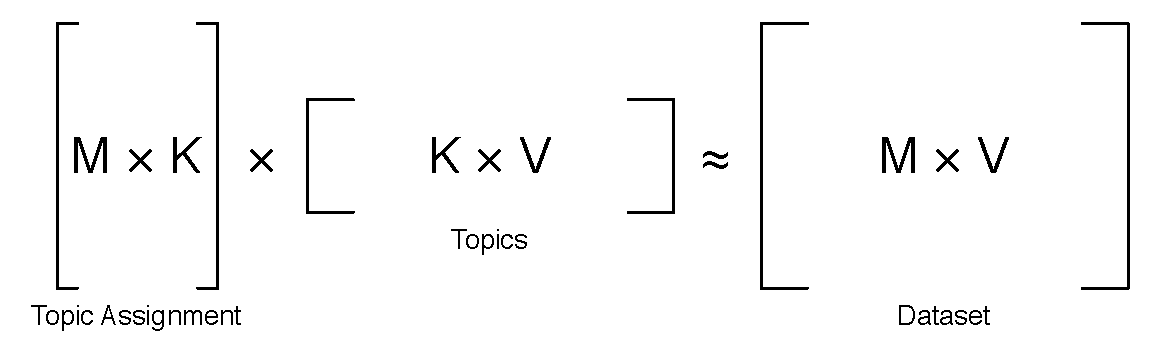
\includegraphics[width=.8\linewidth]{figures/matrix_factorization}
  \end{center}

  \caption{A matrix formulation of finding $K$ topics for a dataset
    with $M$ documents and $V$ unique words.  While this view of topic
    modeling includes approaches such as latent semantic analysis
    (\abr{lsa}, where the approximation is based on \abr{svd}), we
    focus on probabilistic techniques in the rest of this survey.}
  \label{fig:matrix_topics}
\end{figure}
\end{center}

You might notice that we are using the general term ``topic model''.
There are many specific mathematical formulations of topic models, and many algorithms that learn the parameters of those models from data.
Although we will focus on particular models and algorithms, we choose our terminology in order to emphasize that the similarities between formulations, models, and algorithms are often greater than their differences.

\index{latent semantic analysis}
Topic modeling began with a linear algebra approach~\citep{deerwester-90} called
latent semantic analysis (\abr{lsa}): find the best low rank approximation of a
document-term matrix (Figure~\ref{fig:matrix_topics}).  While these approaches
have seen a resurgence in recent years~\citep{anandkumar-12:lda,arora-13}, we
focus on probabilistic approaches~\citep{hofmann-99,papadimitriou-00,blei-03},
which are intuitive, work well, and allow for
easy modification (as we see later in many of our later chapters).

\index{latent Dirichlet allocation}
\index{probabilistic latent semantic analysis}
The two foundational probabilistic topic models are latent Dirichlet
allocation~\citep[\abr{lda}]{blei-03} and probabilistic latent
semantic analysis~\citep[\plsa{}]{hofmann-99}.  We describe the
former in significant detail in Chapter~\ref{sec:lda}, but we want to
take a moment to address some of the historical connection between
these two models.

\plsa{} was historically first and laid the foundation for \abr{lda}.
\plsa{} was used extensively in many applications such as information
retrieval.  However, this survey focuses on \abr{lda} because more
researchers have not just \emph{used} \abr{lda}---they have also
\emph{extended} it.  \abr{lda} is not just widely used, but it's also
widely modified.  Because of these prolific modifcations, we feel it
is more important to focus on the mechanics of \abr{lda}, which many
researchers have used as the foundations of new models.  However, as
we explain below (Chapter~\ref{sec:plsa-vs-lda}), the similarities
between \plsa{} and \abr{lda} outweigh the differences.

\begin{figure}
\small
\rowcolors{2}{gray!25}{white}
  \begin{tabular}{cccc}
\hline
\rowcolor{gray!50}
 & & Example & Example \\
\rowcolor{gray!50}
    Distribution & Density & Parameters & Draws \\
    \hline \hline
    Gaussian  & $\frac{1}{\sqrt{2 \sigma^2 \pi}} e^{- \frac{(x-\mu)^2}{2 \sigma^2}}$ & $\mu=2, \sigma^2=1.1$ & $x=2.21$\\
    Discrete  & $\prod_i \phi_i^{\ind{w=i}}$ & $\phi=\begin{bmatrix}
           0.1 \\
           0.6 \\
           0.3 
         \end{bmatrix}$
                                                & $w=2$ \\
   Dirichlet & $\frac{\prod_{i=1}^K \Gamma(\alpha_i)}{\Gamma \left( \sum_{i=1}^K \alpha_i \right)} \prod_{i=1}^K \theta_i^{\alpha_i - 1} $ & $\alpha = \begin{bmatrix}
           1.1 \\
           0.1 \\
           0.1 
         \end{bmatrix}$  & $\theta = \begin{bmatrix}
           0.8 \\
           0.15 \\
           0.05 
         \end{bmatrix}$ \\
     \hline
  \end{tabular}
  \caption{Examples of probability distributions used in the
    generative stories of topic models.  In the case of the discrete
    draw, $w=2$ denotes that the second element (the one with
    probability $0.6$) was drawn.}
  \label{fig:distribution_examples}
\end{figure}

Despite the similarity in terms, the meaning of ``topic'' in topic modeling is distinct from the meaning in many information retrieval settings.
There is a substantial and well-developed field of topic detection and tracking~\citep{allan-02}.
In \abr{tdt}, a topic is usually closer to an event or an individual story.
In contrast, topic models tend to identify more abstract latent factors.
For example, a \abr{tdt} topic might include an earthquake in Haiti, whereas a topic model might represent the same event as a combination of topics such as Haiti, natural disasters, and international aid.

There has been some work on using topic models to detect emerging events by searching for changes in topic probability~\citep{alsumait-08}.
But these methods tend to identify mainly the fact that an event has occurred, without necessarily identifying the specific features of that event.
Other work has found that more lexically specific methods than topic
models are best for identifying memes and viral
phrases~\citep{leskovec-09}. \\


\subsection{Probabilistic Building Blocks}
\label{sec:intro_building_blocks}

In probabilistic models we want to find values for unobserved model variables that do a good job of explaining the observed data.
The first step in inference is to turn this process around, and assert a way to generate data given model variables.
Probabilistic models thus begin with a generative story: a recipe listing a sequence of random events
that creates the dataset we are trying to explain.
Figure~\ref{fig:distribution_examples} lists some of the key players in these
stories, how they are parameterized and what samples drawn from these distributions look like.  We will
briefly discuss them, as we will use them to build a wide variety of topic models later.

\paragraph{Gaussian} If you know any probability distribution already,
it is (probably) the
Gaussian.  This distribution does not have a role in the most basic topic models that we will
discuss here, but it will later (e.g., Chapter~\ref{ch:css}).  We
include it because it is a useful point of comparison against the other
distributions we {\em are} using (since it is perhaps the easiest to understand and best
known). A Gaussian is a distribution over all real numbers (e.g., $0.0, 0.5,
-4.2, \pi$, \dots).  You can ask it to spit out a number, and it will give you
some real number between negative infinity and positive infinity.  But not all
numbers have equal probability.  Gaussian distributions are parameterized by a
mean $\mu$ and variance $\sigma^2$.  Most samples from the distribution will be
near the mean $\mu$; how close is determined by the variance: higher variances
will cause the samples to be more spread out.

\paragraph{Discrete}

While Gaussian distributions are over a continuous space, documents are
combinations of discrete symbols, usually word tokens.\footnote{An emerging trend in natural language
  processing research is to view words as embedded in a continuous space. We
  discuss these ``representation learning'' approaches and their connection to
  topic modeling in Chapter~\ref{ch:conc}, but even then models are still defined over a discrete set of words.}   Thus, we need a distribution
over discrete sets.

A useful metaphor for thinking about discrete distributions is a weighted die.
The number of faces on the die is its dimension, and each face is associated with a distinct
outcome.  Each face has its own probability of how likely that outcome is;
these probabilities are the parameters of a discrete distribution
(Figure~\ref{fig:distribution_examples}).

Topic models are described by discrete distributions (sometimes called
multinomial distributions) that describe the connection between words and topics (the first half) and topics and documents (the second half).  A distribution
over words is called a topic distribution; each of the topics gives
higher weights to some words more than others (e.g., in Topic 9 from
the Enron corpus, ``state'' and ``california'' have higher probability
than other words).  Each document also has an ``allocation'' for each
topic: documents are about a small handful of topics, and most
documents have very low weights for most of the possible topics.

\paragraph{Dirichlet}

Although discrete distributions are the star players in topic models, they are
not the end of the story.  We often begin with Dirichlet distributions.
Just as Gaussians produce real numbers and discrete distributions produce symbols from a finite set, Dirichlet distributions produce probability vectors that can be used as the parameters of discrete distributions.
Like the Gaussian distribution, they have parameters analogous to a mean and
variance.  The mean is called the ``base measure'' $\tau$ and is the expected
value of the Dirichlet distribution: the values you would get if you averaged many draws from the
Dirichlet.  The concentration parameter $\alpha_0$ controls how far away individual draws are from the base measure.
Note that we often combine these parameters into a single value for each dimension: $\alpha_k = \alpha_0 \tau_k$.

\begin{center}
\begin{figure}
  \centering
  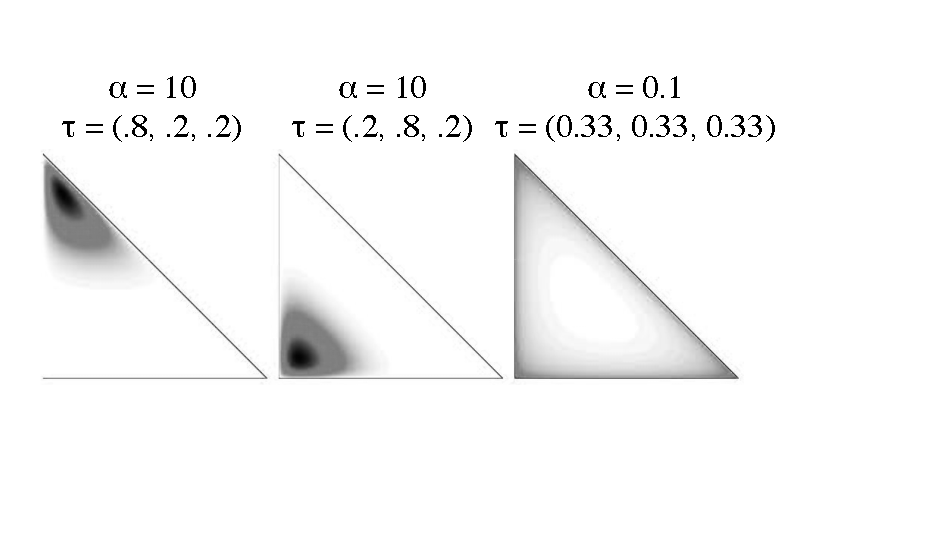
\includegraphics[width=.8\linewidth]{figures/dirichlet}
  \caption{Given different Dirichlet parameters, the Dirichlet
    distribution can either be informative (left, middle) or sparse
    (right).  Sparse distributions encourage distributions to favor
    only a small number of elements but do not care which ones.  This
    is consistent with our intuitions of how documents are written:
    they are only about a few things, and topics contain only a
    handful of words.}
  \label{fig:dirichlet_sparsity}
\end{figure}
\end{center}


If $\alpha_0$ is very large, then the draws from a Dirichlet will be very close to
$\tau$ (Figure~\ref{fig:dirichlet_sparsity}, left).  If $\alpha_0$ is small, however,
something more interesting happens: the discrete distributions become sparse
(Figure~\ref{fig:dirichlet_sparsity}, right).  A sparse distribution is a
distribution where only a few values have high probability and all other values are small.

Because topic models are meant to reflect the properties of real documents, modeling sparsity is important.  When a person sits down to write a document, they only
write about a handful of the topics that they could potentially use.  They do not write about every possible topic, and the sparsity of Dirichlet distributions is the probabilistic
tool that encodes this intuition.

There are several important special cases of the Dirichlet distribution.
If the base measure $\tau$ is uniform, we call the resulting distribution {\em symmetric}.
This case is appropriate when we do not expect any one element to be, on average, more likely than any other element across all samples from the distribution.
In the symmetric case the  distribution has only one parameter, the concentration $\alpha_0$.
If the base measure is uniform and the concentration parameter $\alpha_0$ is equal to the number of dimensions $K$ (or, equivalently, $\alpha_k = 1.0$ for all $k$), the distribution is uniform, placing equal probability on all $K$-dimensional probability distributions.


\section{Latent Dirichlet Allocation}
\label{sec:lda}

We now have all the tools we need to tell the complete story of the most popular topic model: latent Dirichlet allocation~\citep{blei-03}.  Latent
Dirichlet allocation\footnote{The name \abr{lda} is a play on \abr{lsa}, its
  non-probabilistic forerunner (latent semantic analysis).  Latent because we
  use probabilistic inference to infer missing probabilistic pieces of the
  generative story.  Dirichlet because of the Dirichlet parameters encoding
  sparsity.  Allocation because the Dirichlet distribution encodes the prior for
  each document's allocation over topics.} posits a ``generative process'' about
how the data came to be.  We assemble the probabilistic pieces to tell
this story about generating topics and how those topics are used to create
diverse documents.

\paragraph{Generating Topics}

The first part of the story is to create the topics.  The user specifies that
there are $K$ distinct topics.  Each of the $K$ topics is drawn from a Dirichlet
distribution with a uniform base distribution and concentration parameter
$\lambda$: $\phi_k \sim \dir{\lambda {\bm u}}$.  The discrete distribution
$\phi_k$ has a weight for \emph{every} word in the vocabulary.

However, when we summarize topics (as in
Figure~\ref{fig:enron_topics}), we typically only use the top (most probable) words of
a topic.  The lower probability words are less relevant to the topic
and thus are not shown.

\paragraph{Document Allocations}

Document allocations are distributions over topics for each document.  This
encodes what a document is about; the sparsity of the Dirichlet distribution's
concentration parameter $\alpha_0$ ensures that the document will only be about a
few topics.  Each document has a discrete distribution over topic: $\theta_d \sim
\dir{\alpha {\bm u}}$.

\paragraph{Words in Context}

Now that we know what each document is about, we need to actually create the
words that appear in the document.  We assume\footnote{It is possible to model
  this in the generative story as well, e.g., with a Poisson distribution.
  However, we often do not care about document \emph{lengths}---only what the
  document is about---so we can usually ignore this part of the story.} that
there are $N_d$ words in document $d$.  For each word $n$ in the
document $d$, we first choose a {\bf topic assignment} $z_{d,n} \sim
\disc{\theta_d}$.  This is one of the $K$ topics that tells us which topic the
word token is from, but not what the word is.

To select which word we will see in the document, we draw from a discrete
distribution again.  Given a word token's topic assignment $z_{d,n}$, we draw from that
topic to select the word: $w_{d,n} \sim \phi_{z_{d,n}}$.  The topic assignment
tells you what the word is about, and then this selects which distribution over
words we use to generate the word.  % (Figure~\ref{fig:generative-ex}).

For example, consider the document in Figure~\ref{fig:enron_doc}.  To
generate it, we choose a distribution over all of the topics.  This is
$\theta$.  For this document, the distribution favors Topic~9 about
\underline{California}.  The value for this topic is higher than any other topic.  For
each word in the document, the generative process chooses a topic
assignment $z_n$.  For this document, any topic is theoretically possible, but we expect that most of those will be Topic~9.

Then, for each token in the document, we need to choose which word type will appear.  This
comes from Topic~9's distribution over words (multiple topics have
word distributions shown in Figure~\ref{fig:enron_topics}).  Each is a
discrete draw from the topic's word distribution, which makes words
like ``California'', ``state'', and ``Sacramento'' more likely.

It goes without saying that the generative story is a fiction~\citep{box-87}.
Nobody is sitting down with dice to decide what to type in on their keyboard.
We use this story because it is \emph{useful}.  This fanciful story about randomly
choosing a topic for each word can help us because if we assume this generative
process, we can work backwards to find the topics that explain how a document
collection was created: every word, every document, gets associated with these
underlying topics.

This simple model helps us order our document collection: by assuming this story, we
can discover \emph{topics} (which certainly do not exist) so we can understand
the common themes that people use to write documents.  As we will see in later
chapters, slight tweaks of this generative story allow us to uncover more
complicated structures: how authors prefer specific topics, how topics change
over time, or how topics can be used across languages.

\section{Inference}

Given a generative model and some data, the process of uncovering the hidden
 pieces of the probabilistic generative story is called \emph{inference}.  More
concretely, it is a recipe for generating algorithms to go from data to
\emph{topics that explain a dataset}.

There are many flavors of algorithms for posterior inference: message
passing~\citep{zeng-13}, variational inference~\citep{blei-03},
gradient descent~\citep{hoffman-10}, and Gibbs
sampling~\citep{griffiths-04}.  All of these algorithms have their
advocates and reasons you should use them.  In this survey, we focus
on Gibbs sampling, which is simple, intuitive, and---with some clever
tricks specific to topic models---fast~\citep{yao-09}.  (We discuss
variational inference in Chapter~\ref{ch:building}.)

We present the results of Gibbs sampling without derivation,
which---along with the history of its origin in statistical
physics---are well described elsewhere.\footnote{We recommend
  \citet{resnik-09} for additional information on derivation.} We use
a variety of Gibbs sampling called \emph{collapsed} Gibbs sampling,
which allows inference to side-step some of the pieces of the
generative story: instead of explicitly representing the parameters of
a discrete distribution, distinct from any observations drawn from
that distribution, we represent the distribution solely through those
observations.  We can then recreate the topic and document
distributions through simple formulas as they are needed.

\subsection{Random Variables}

\paragraph{Topic Assignments}

Since every individual token is assumed to be generated from a single topic,
we can consider the {\em topic assignment} of a token as a variable.  For example,
an instance of the word ``compilation'' might be in a \underline{computer} topic in one
document and in an \underline{arts} topic in another document.  Because each token has its own
topic assignment, it is even possible that the
same word might be assigned to different topics in the same document.
To estimate \emph{global} properties of the topic model we use aggregate statistics derived from these token-level topic assignments.

\paragraph{Document Allocation} The document allocation is a distribution over
the topics for each document; in other words, it says how popular each topic is
in a document.  If we count up how often a document uses a topic, this gives us
an idea of the popularity.  Let's define $\dc{d}{i}$ as the number of times
document~$d$ uses topic~$i$.  Clearly, this is larger for more popular topics;
however, it is not a probability because it is larger than one.  We can make it a
probability by dividing by the number of words in a document
\begin{equation}
\frac{\dc{d}{i}}{\sum_k \dc{d}{k}},
\label{eq:theta_ml}
\end{equation}
but this is problematic because it can sometimes give us zero and ignores the
influence of the Dirichlet distribution; a better estimate is\footnote{To be
  technical, Equation~\ref{eq:theta_ml} is a maximum likelihood estimate and
  Equation~\ref{eq:theta_map} is the maximum \textit{a posteriori}, which
  incorporates the influence of both the prior and the data.}
\begin{equation}
\theta_{d,i} \approx \frac{\dc{d}{i} + \alpha_i}{\sum_k \dc{d}{k} + \alpha_k}.
\label{eq:theta_map}
\end{equation}
It is important that this is never zero because we do not want it to rule out the possibility
that a topic is used in a particular document.  This helps the sampler
explore more of the possible combinations.

\paragraph{Topics}

Each topic is a distribution over words.  To understand what a topic is about,
we look at the profile of all of the tokens that have been assigned to that
topic.  We estimate the probability of a word in a topic as
\begin{equation}
\phi_{i,v} \approx \frac{\tc{i}{v} + \beta_v}{\sum_w \tc{i}{w} + \beta_w},
\label{eq:phi_map}
\end{equation}
where $\beta$ is the Dirichlet parameter for the topic distribution.

\subsection{Algorithm}

The collapsed Gibbs sampling algorithm for learning a topic model is
only based on the topic assignments, but we will use our estimates for
the topics $\phi_k$ and the documents $\theta_d$ discussed above.  We
begin by setting topic assignments randomly: if we have $K$ topics,
each word has equal chance to be associated with any of the topics.
These topics will be quite bad, looking like noisy copies of the
overall corpus distribution. But we will improve them one word at a
time.

The algorithm proceeds by sweeping over all word tokens in turn over and over.
At each iteration we change the topic assignments for each word in a way the reflects the
underlying probabilistic model of the data.  On average, each pass over the data makes the
topics slightly better until the model reaches a steady state.  There is no easy way
to tell when such a steady state has been reached, but eventually the topics will ``converge'' to something reasonable and you can consider yourself done.

The equation for the probability of assigning a word to a particular topic
combines information about words and about documents\footnote{To be theoretically correct, it is important
not to include the count associated with the token you are currently sampling in
these counts, which becomes more clear if the probability is written as
$p(z_{d,n}=j\,|\,z_{d,1}\dots z_{d,n-1},z_{d,n+1}\dots z_{d,N_d}, w_{d,n})$ to
show the dependence on the topic assignments of \emph{all other} tokens but not
this token.}
\begin{align}
p(z_{d,n}=i \g \dots) = \theta_d
\phi_ji= \left(\frac{\dc{d}{i} + \alpha_i}{\sum_k \dc{d}{k} + \alpha_k} \right) \left( \frac{\tc{i}{w_{d,n}} + \beta_v}{\sum_w \tc{i}{w} +
    \beta_w} \right).
\label{eq:sampling}
\end{align}
Computing this value for each topic will result in a probability distribution over the topic assignment for this word token, given all the other topic assignments.  The next step is to randomly choose one of those indices with
probability proportional to the vector value.  You now assign that word to the
topic, update $\dc{d}{\cdot}$ and $\tc{\cdot}{w_{d,n}}$, and move on to the next word and repeat.
The two terms provide two ``pressures'', for global and local coherence. Sparsity in the topic-word distributions encourages tokens of the same word type to be assigned to a small number of topics,  regardless of where they occur. Sparsity in the document-topic distributions encourages tokens in the same document to be assigned to a small number of topics, regardless of what type they are.
For example, knowing that a word is ``compilation'' narrows down the
number of potential topics considerably, but leaves ambiguity: is it
\underline{computer} compilation or a \underline{music} compilation? Knowing that the word occurs in a document with many other words in the \emph{arts} topic resolves this ambiguity, leaving the \emph{arts} topic as the most probable assignment.

At the very end of the algorithm, we can use the estimates of each topic
(Equation~\ref{eq:phi_map}) to summarize the main themes of the corpus and the
estimates of each document's topic distribution (Equation~\ref{eq:theta_map}) to
start exploring the collection automatically (Chapter~\ref{ch:ir}) or with a
human in the loop (Chapter~\ref{ch:viz}).

The algorithm that we have sketched here is the foundation of many of the more
advanced models that we will discuss later in the survey.  While we will not describe
the algorithms in detail, we will occasionally make reference to this sketch to
highlight challenges or difficulties in implementing topic models.

\subsection{Plate Diagrams}
\label{sec:plate}

Plate diagrams provide a shorthand for quickly explaining which random
variables are associated with each other.  If you look up many of the
references used in this survey, you'll likely see plate diagrams (we
also use a plate diagram later in Figure~\ref{fig:ptm-simplified}).  

\begin{figure}
  \begin{center}
  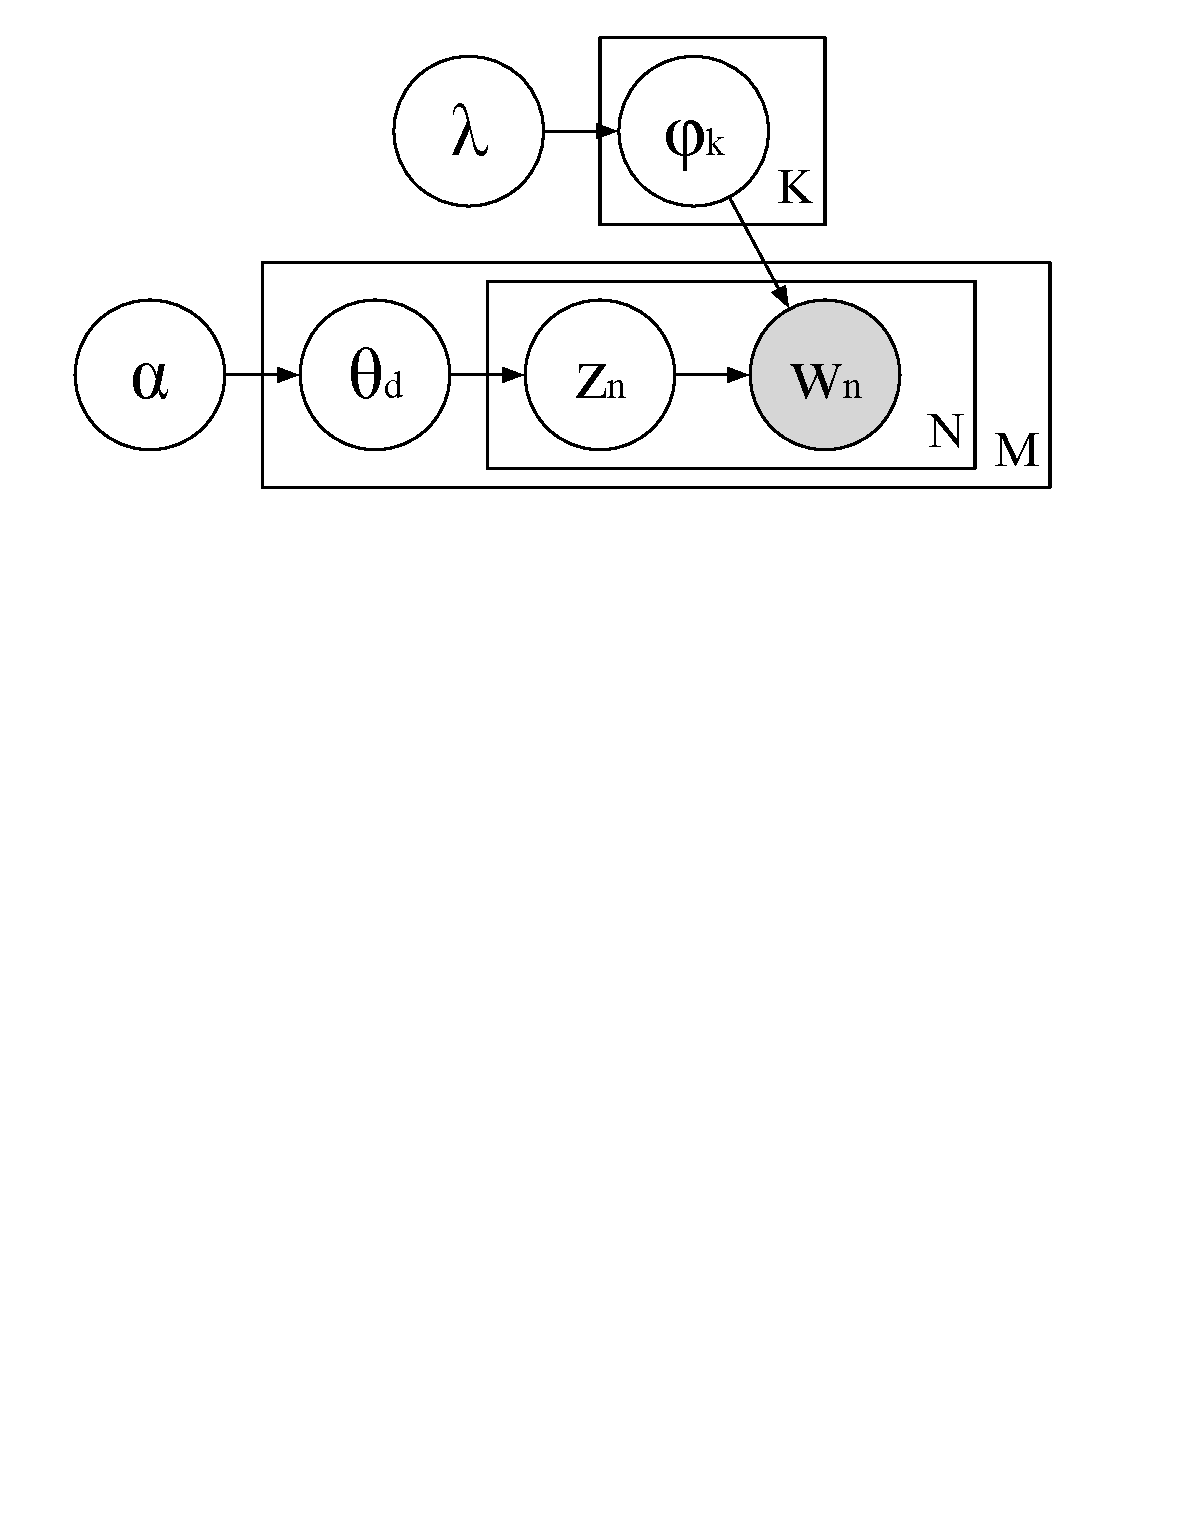
\includegraphics[width=0.7\linewidth]{figures/lda_plate}
  \end{center}
  \caption{Plate diagram for \abr{lda}.  Nodes show random variables,
    lines show (possible) probabilistic dependence, rectangles show
    repetition, and shading shows observation.}
  \label{fig:plate-lda}
\end{figure}

Let's begin with a plate diagram for \abr{lda}
(Figure~\ref{fig:plate-lda}).  You can compare these to the generative
story in Chapter~\ref{sec:lda}.  All of the random variables are
there, each in its own circle.  The lines between random variables
tell more of the story.  You can see that if a random variable is
conditioned on another, there is a line going from the variable that
is \emph{conditioned on} {\bf to} the variable that is
\emph{conditionally dependent}.  For example, a word depends on the
token assignment $z_{d,n}$ and a topic $\phi_k$, so there are lines
from both.

You can think about the rectangular boxes as repetition.  The letter
in the bottom right of the box shows how often what's inside the box
is replicated.  There is a box for each document (there are $M$ in
total) and each token (the box of words is inside the box for
documents, so there are many more tokens than documents).

When a variable is shaded, this means that it is observed.  These are
the data we start with.  The unshaded variables must either be
inferred (e.g., topics $\phi$) or are hyperparameters that must be set
or inferred (e.g., Dirichlet parameter $\alpha$).

Plate diagrams allow a reader to quickly see a ``family resemblance''
between related models, and once someone has become fully immersed in
topic models, it's often possible to at a glance understand a model
from its plate diagram.  However, plate diagrams are imperfect; they
lack some of the key information you need to understand the model.
For instance, the exact probabilistic relationship between variables
is underspecified.

\subsection{What's so Great about Dirichlet?}
\label{sec:plsa-vs-lda}

Now that we have described what \abr{lda} is, we can return to its
history.  What is the innovation that separates \abr{lda} from
\plsa{}, its predecessor?  Na\"ively, the difference is changing an
``s'' to a ``d'' (i.e., changing p\abr{l{\bf S}a} to \abr{l{\bf
    D}a}).  The deeper story is about as consequential.

Instead of having a Dirichlet prior over $\theta$, \plsa{} assumes
that $\theta$ is simply a multinomial parameter.  In practice, this
means that documents aren't encouraged to focus on a limited number of
topics and often ``spread out'' to have small weights for many
different topics.  In theory, this means that there isn't as sound a
generative story for how a document came to be: you can't run the
generative process forward from scratch if you must have $\theta$ as a
parameter to start with.

These differences are relatively minor.  \abr{lda} has slightly easier
inference---particularly when it comes to tweaking the model---which
has caused it to become the more popular of the two models.  Thus, we
will focus on comparing models to \abr{lda}.  This is
not to diminish from \plsa{} and its incontrovertible place in the
literature, it helps us present a more unified narrative for our reader.

\subsection{Implementations}

Hopefully the previous algorithm sketch has convinced you that implementing
topic models is not a Herculean task; most skilled programmers can complete a
reasonable implementation of topic models in less than a day.  However, we would
suggest not trying to implement basic \abr{lda} if you just want the
output of a topic model, as there are many solid
implementations that help users get to useful results more quickly, particularly
as topic models often require extensive preprocessing.

Mallet is fast and is a widely used implementation in Java~\citep{mallet}.  This
is where you should probably start, in our biased opinion.  It runs in Java, uses
highly-optimized Gibbs sampling implementations, and can work from a variety of
text inputs.  It is well documented, mature, and runs well on a multi-core
machine, allowing it to process up to millions of documents.  Variational
inference is the other major option~\citep{blei-03,vw}, but often requires a
little more effort for new users to get a first result.

However, not all users are comfortable with Java; there are many
implementations available on other platforms and in many programming
languages.\footnote{There are so many and they change so quickly that
  we're reluctant endorse specific ones here.}  Many of these
implementations are well-built, but it may be worthwhile checking
whether they have all of the features of mature implementations like
Mallet so that you know what (if anything) you're missing.

% Smola, Amr
However, if your corpus is truly large, it may be worthwhile
considering techniques that can be parallelized over large computer
clusters.  These techniques can be based on variational
inference~\citep{Narayanamurthy-11,zhai-12} or on
sampling~\citep{newman-08}.

While these implementations allow you to run \emph{specific} topic
models, other frameworks allow you to specify arbitrary generative
models.  This allows for quick prototyping of topic models and
integrating topic models with other probabilistic frameworks like
regression or collaborative filtering.  Examples of these general
frameworks include Stan~\citep{stan-software:2014},
Theano~\citep{theano}, and Infer.net~\citep{InferNET14}.

If you cannot find the specific model that you want among these
existing software packages, the flexibility and simplicity of topic
models and inference makes it relatively simple to adapt topic models
to model specific phenomena (as we describe in following chapters).

\section{The Rest of this Survey}

In each of the following chapters, we focus on an application of topic
models, gradually increasing the complexity of the underlying models.
The chapters do occasionally refer to each other, but a reader should
be able to read each of the chapters independently.

The next chapter returns to the distinction between high level
overviews and finding a needle in a haystack.  We show how a high
level overview can help users and algorithms find documents of
interest.  We show how a high level overview can help
algorithms (Chapter~\ref{ch:ir}) and users (Chapter~\ref{ch:viz}) find documents
of interest.

These tools help enable new applications of topic models: how
understanding newspapers (Chapter~\ref{ch:nonfiction}) reveals the
march of history, how the corpus of writers of fiction
(Chapter~\ref{ch:fiction}) illuminates societal norms, how the
writings of science reveal innovation (Chapter~\ref{ch:sci}), or
how politicians' speeches (Chapter~\ref{ch:css}) reveal schisms in
political organizations.

Finally, the survey closes with thoughts about how interested
researchers can start building their own topic models
(Chapter~\ref{ch:building}) and how topic models may change in the
future (Chapter~\ref{ch:conc}).

\chapter{Information Retrieval}
\label{ch:ir}

Topic models explore and summarize document collections, without knowing users' information need. In the contrary, traditional information retrieval (IR) systems aim to retrieve relevant documents given users' information need. Users start with their information need in the form of queries, and early IR systems treat both the query and documents as ``bag of words'', retrieve and rank the documents by measuring the word overlap between queries and documents.

\jbgcomment{It would be good to contrast a little bit with the role that topic models serve in exploring document collections (discussed in the intro); i.e., you don't know what you're looking for.  This chapter focuses instead on when you do know what you're looking for (in the form of a query).  We may even want to call this ``traditional information retrieval'' or ``query-based IR''. \yhcomment{connected a little.}}

However, the ability of this direct and simple matching is always limited. Words with similar meaning or in different forms should also be considered as matched instead of being ignored. \textbf{Language modeling} has been one of the most popular frameworks to capture such semantic relationships. Also, humans would also use background knowledge to interpret and understand the queries and ``add'' missing words~\citep{wei-07}, which provides another way often referred as \textbf{query expansion} to improve the retrieval and ranking results.

Both directions can be pursued by learning and discovering the semantic relations between words and further the semantic relations between queries and documents. Topic models, which describe each topic using weighted words and model each document as a distribution over all topics, provides a semnatic relations between query words and documents~\citep{deerwester-90,hofmann-99a}. Such semantic relations can be applied to smoothing the language models, or introducing related words in query expansion. This chapter focuses on how to apply topic models in document language modeling \citep{Lu-2011,wei-06} and query expansion~\citep{Park-2009,Andrzejewski-2011} to further improve the ranking results of information retrieval. We start with a brief review of the traditiona information retrieval framework.

\jbgcomment{how? \yhcomment{Added.}} 

\section{Document Language Modeling in IR}

The language modeling approach~\citep{croft-03,PonteCroft,song-99} is one of the main frameworks for using topic models in IR systems, since it has been shown to be effective probabilistic framework for studying information retrieval problem~\citep{PonteCroft,berger-99}.

A statistical language model is to estimate the probability of word sequences, denoted as $p(w_1,w_2,\cdots,w_n)$. In practice, the statistical language model is often approximated by N-gram models. A unigram model assumes each word in the sequence is independent, and is denoted as,
\begin{align}
p(w_1,w_2,\cdots,w_n) = p(w_1)p(w_2) \cdots p(w_n)
\end{align}
A trigram model assumes the probability of the current word only depends on the previous two words, and it is represented as,
\begin{align}
p(w_1,w_2,\cdots,w_n)=p(w_1)p(w_2|w_1)p(w_3|w_1,w_2)\cdots p(w_n|w_{n-2},w_{n-1})
\end{align}

\jbgcomment{would be good to add backpointers to previous chapter. \yhcomment{Not sure which part in prevous chapter you mean.}}

In the application of information retrieval, the queries are generated by a probabilistic language model based on a document~\citep{zhai-01}. More specifically, each document is viewed as a language sample, and a language model for each document is estimated based on document terms. Then the probability of generating the query is estimated by each document language model. The probability of a query is computed by multiplying the probabilities of generating each query term using different document language model, and the documents are ranked based on the probability.

Given a document sample $d$, a straightforward way to estimate the probability of generating a word $w$ is to use the maximum likelihood estimation as,
\begin{align}
p_{\texttt{ml}}(w|d) = \frac{n_{d,w}}{n_{d,\cdot}}
\label{eq:ir_mse}
\end{align}
where $n_{d,w}$ is the term frequency of word $w$ in document $d$, and $n_{d,\cdot}$ is the total number of tokens in document $d$. Then the probability of the given query $q$ can be computed by,
\begin{align}
p(q|d) = \prod_{w \in q} p(w|d) = \prod_{w \in q} \frac{n_{d,w}}{n_{d,\cdot}}
\end{align}

Then the documents are ranked based on this probability. Higher probability implies the corresponding document is more relevant to the given query~\citep{song-99}. However, a document is often too small to cover all the terms in the query. The probability of a missing term is zero, which means the probability of the whole query is zero and causes problems for ranking documents. 

This data sparsity problem can be fixed by smoothing, which allocates some non-zero probability to the missing terms. In fact, topic models provide a unique way to extract the word probabilities given the corpus, which can be used to smooth doucument language models.
In this section, we summarize two simple smoothing methods, and then introduce how topic models are applied to smooth document language models in the next section.

%\subsection{Smoothing Document Language Models}

\jbgcomment{Is this important to talk about here?  I worry that it might be a distraction.  will this connect directly to topic models? \yhcomment{Yes, it is important. Topic models are applied to document LM in forms of smoothing. Simplified and added more connections. }}

There are two major directions for smoothing: \textbf{interpolation}~\citep{Jelinek-1980,mackay95dirichlet,Ney-1994,PonteCroft,zhai-01} and \textbf{backoff}~\citep{katz-87,song-99}. The interpolation-based method discount the counts of the seen words and distribute the extra counts to both seen words and unseen words. An alternative backoff smoothing strategy trusts the maximum likelihood estimation for high count words, discounts and  redistributes mass only for the less common words~\citep{zhai-01}.

Here we introduce two popular and simple interpolation smoothing methods, which are further used by topic models to smooth document language models.

\paragraph{Jlinek-Mercer method}

The Jlinek-Mercer method~\citep{Jelinek-1980} is a linear interpolation of the maximum likelihood model in a document with the model based on the whole corpus, and a coefficient $\lambda$ is used to combine the two parts.
\begin{align}
p(w|d) = (1 - \lambda) p_{\texttt{ml}(w|d)} + \lambda p(w|\mathcal{C})
\end{align}
where $\mathcal{C}$ denotes the whole corpus. This simple mixture solves the data sparsity problem. For terms that occur in the document $d$, the maximum likelihood estimator (Equation~\ref{eq:ir_mse}) is not accurate given the limited size of a document, thus it is smoothed with the more reliable corpus level probability. For the missing terms in the document $d$, the probability is not zero any more, but fall back to the corpus level probability. This smoothing method has been explored by \cite{PonteCroft} and \cite{song-99} in information retrieval task, except \cite{PonteCroft} explored a weighted product version instead of a linear interpolation.
\begin{align}
p(w|d) = p_{\texttt{ml}}(w|d)^{(1 - \lambda) } \times p(w|\mathcal{C})^{\lambda}
\label{eq:lm-jr}
\end{align}
But in general, the linear interpolation is more popular since the resulting probability is still normalized~\citep{song-99}.

\paragraph{Bayesian Smoothing using Dirichlet Priors}

A language model can be viewed as a multinomial distribution, thus it can be smoothed by applying the Dirichlet distribution as the conjugate prior~\citep{mackay95dirichlet}. The smoothing model is adding extra prior count for each word to smooth the probability of unseen words,
\begin{align}
p(w|d) = \frac{n_{d,w} + \mu p(t|\mathcal{C})}{\sum_{v \in V} n_{d,v} + \mu}
\end{align}
where the Dirichlet prior is decided by parameter $\mu$ and the corpus-level probabilities $p(v|\mathcal{C})$ as follows,
\begin{align}
(\mu p(v_1 | \mathcal{C}), \mu p(v_2 | \mathcal{C}), \cdots, \mu p(v_n | \mathcal{C}))
\label{eq:lm-bs}
\end{align}

%\paragraph{Absolute Discounting}

%Absolute discounting is to allocate some probability mass from the seen words to the unseen words~\cite{Ney-1994}. Normally, a constant is subtracted from their actual counts for the seen words. This model is given by,
%\begin{align}
%p(w|d) = \frac{\max(n_{d,w} - \delta, 0)}{\sum_{v \in V} n_{d,v}} + \sigma p(w|\mathcal{C})
%\end{align}
%where $\delta \in [0,1]$ is the discount constant and $\sigma = \delta n'_{d,\cdot} / n_{d, \cdot}$, $n_{d, \cdot}$ is the total number of tokens in document $d$, and $n'_{d,\cdot}$ is the number of unique terms in document $d$.

\section{Applying Topic Models to Document Language Models}

Topic models, which model each document as a mixture of topics and each topic as a mixture of words, offer an interesting framework to model documents in information retrieval. \cite{wei-06} introduce Latent Dirichlet Allocation (LDA) to learn the relationship between query words and documents, and the conditional probability of a query word $w$ given a document $d$ is computed as marginalizing all topics,
\begin{align}
p_{\texttt{lda}}(w|d) = \sum_{z=1}^K p(w|z, \hat{\phi}) p(z | \hat{\theta}, d)
\end{align}
where $\hat{\theta}$ is the posterior estimate for the document-topic distribution $\theta$; $\hat{\phi}$ is the posterior estimate for the topic-word distribution $\phi$; $K$ is the total number of topics.

Because topic models learn the semantic relationships between words and documents through learning the hidden topics, and their posterior estimates of document-topic distribution and topic-word distribution are smoothed by the Dirichelet priors, topic models learn a better and smoothed semantic relationship between words and documents. However, the topic models based on documents only lose the direct connection between query words and documents as in the original document language models, but it is a good approach to complement the original document language models. Thus \cite{wei-06} further propose to combine the LDA-based document model with the original smoothed document model~(Equation~\ref{eq:lm-jr}) through a linear interpolation,
\begin{align}
p(w|d) = \omega ((1 - \lambda) p_{\texttt{ml}(w|d)} + \lambda p(w|\mathcal{C})) + (1 - \omega) p_{\texttt{lda}}(w|d)
\end{align}
where $\omega$ is the coefficient which combines the LDA-based document model with the general smoothed language model.

\jbgcomment{I don't know this work as well, but I haven't seen enough here to convince me that this is a good idea.  How does it help performance, why is it a good idea?  \yhcomment{added.}}

Following \cite{wei-06}, \cite{Lu-2011} further evaluate the performance of applying topic models into the document language model framework. Instead of combining with the language model with Jlinek-Mercer smoothing~(Equation~\ref{eq:lm-jr}), \cite{Lu-2011} smooth the document language model with the Bayesian smoothing~(Equation~\ref{eq:lm-bs}), and the final linear combination with topic models is as,
\begin{align}
p(w|d) = \omega \frac{n_{d,w} + \mu p(t|\mathcal{C})}{\sum_{v \in V} n_{d,v} + \mu}  + (1 - \omega) p_{\texttt{lda}}(w|d)
\end{align}

While using different smoothing strategies, both approaches~(\citep{wei-06} and \citep{Lu-2011}) apply topic models to connect the query words with documents through hidden topics. As a result, better semantic relationships between query words and documents can be learned to complement the document language models.

\section{Query Expansion in IR}

The document language models in Information Retrieval~\citep{PonteCroft} have been attempting to model the query generation process based on the document models. However, a big problem is that these models abandon modeling the query-document relevance explicitly~\citep{Lavrenko-2001}, which is very important in traditional Information Retrieval task.

In fact, queries, which are normally brief and using informal languages from users, diverse significantly from the language in documents~\citep{Muller-2009}. This semantic gap or lexical gap can result in poor query-document relevance, even though the document is quite relevant from the users' view point. This is due to users, who add ``missing'' or potentially related words implicitly in their minds and then consider the query-document relevance.

Query expansion simulates the similar process. Query expansion normally analyzes the relationships between the query words and other words, and tries to find potential related words so that the original query is better represented and better query-document relevance can be obtained. This section reviews the classic query expansion frameworks in information retrieval and then we introduce the related works about using topic models for query expansion in the next section.

\subsection{Learning Query-Word Relationships for Query Expansion}

There are two main steps for query expansion. The first step is to find the relationships between queries and words and select the top related words to expand the query. The second step is to apply the expanded queries for ranking and compute the final ranking relevance scores. We start with the first step. Two major directions have been explored: query language model~\citep{zhai-01b} and relevance model~\citep{Lavrenko-2001}.

\paragraph{Query Language Model}

To learn the query-word relationship, \cite{zhai-01b} build up a query language model to estimate the proabbility $p(w|q)$ of a word $w$ given a query $q$. However, it is not easy to learn a good query language model since the query content is too limited.

\cite{zhai-01b} propose to use both the query content and the relevant documents (sometimes referred as feedback documents or clicked documents) to estimate the query language model. Let $\hat{\theta}_{\mathcal{F}}$ be the estimated query language model based on the relevant documents, the combined query model $\hat{\theta}_{Q'}$ can be computed by,
\begin{align}
\label{eq:qlm-comb}
\hat{\theta}_{Q'} = (1 - \mu)\hat{\theta}_{Q} + \mu \hat{\theta}_{\mathcal{F}}
\end{align}

A simple way to estimate the feedback query model $\hat{\theta}_{\mathcal{F}}$ is a unigram language model $\theta$ which generates each word in $\mathcal{F}$ independently. However, most documents contain not only the query relevant information, but also the background information. As a result, \cite{zhai-01b} propose to generate a relevant document by a mixture model, which combines a query model $p(w|\theta_Q)$ with a collection language model $p(w|\mathcal{C})$. Thus the log-likelihood of the relevant document is,
\begin{align}
\log p(\mathcal{F}|\theta) = \sum_i \sum_w c(w, d_i) \log((1-\lambda)p(w|\theta_Q) + \lambda p(w|\mathcal{C}))
\end{align}
where $c(w, d_i)$ is count of word $w$ in document $d$. The related parameters $\theta$ are estimated by the EM algorithm (more details can be found in \cite{zhai-01b}). By combing with the information from the relevant documents, the query language model is more robust, thus query-word relationships are better represented.

\paragraph{Relevance Model}

Different from the query language model approach~\citep{zhai-01b}, \cite{Lavrenko-2001} assume both the query and the relevant documents are random samples from an unknown relevance model $R$. Given the query $q$, they approximate the probability $p(w|R)$ based on the observed query $q$ as the following,
\begin{align}
p(w|R) \approx p(w|q) = \frac{p(w,q)}{p(q)}
\end{align}

To estimate the joint probability $p(w,q)$, \cite{Lavrenko-2001} assumes the word $w$ and the query $q$ are sampled independently from the same distribution, e.g., from a unigram distribution, then the joint probability can be computed as,
\begin{align}
p(w, q) = \sum_{D \in \mathcal{C}} p(D) p(w,q | D) = \sum_{D \in \mathcal{C}} p(D) p(w|D) p(q | D)
\end{align}

Then the multinomial distribution $p(w|q)$ for a given query $q$ can be computed as follows,
\begin{align}
\label{eq:rm_qe}
p(w|q) = \frac{p(w, q)}{p(q)} = \sum_{D \in \mathcal{C}} p(w|D) p(D|q)
\end{align}

Both the query language model and the relevance model capture the relationship between the query and other words, based on which the top related words can be selected for query expansion.

\subsection{Ranking Relevance with Query Expansion}

Given the related words for query expansion, the next question is how to apply the expanded queries for computing the final ranking relevance score. The combination can happen either before or after the relevance score is computed.

\cite{zhai-01b} combine the expanded query language model $\hat{\theta}_{\mathcal{F}}$ with the original query language model $\hat{\theta}_{Q}$ as one query language model $\hat{\theta}_{Q'} $~(Equation~\ref{eq:qlm-comb}). Given a query $q$ generated from the expanded query model $p(q|\hat{\theta}_{Q'})$, and a document $d$ generated from a document model $p(d|\hat{\theta}_D)$, they compute the KL-divergence of document $d$ with respect to query $q$ as the final relevance score:
\begin{align}
D(\hat{\theta}_{Q'} || \hat{\theta}_D) = -\sum_w p(w|\hat{\theta}_{Q'}) \log p(w | \hat{\theta}_D) + \texttt{cons}(q)
\end{align}

Different from \cite{zhai-01b}, \cite{Lavrenko-2001} compute the relevance score using the original query and the expanded query respectively, and then linearly combine the two scores. Thus the final query-document relevance $\hat{s}_d(q)$ is computed as,
\begin{align}
\label{eq:rm_qe_comb}
\hat{s}_d(q) = \mu s_d(e) + (1-\mu)s_d(q)
\end{align}
where $s_d(q)$ is the relevance between the original query $q$ and documents $d$, and $s_d(e)$ is relevance between the expanded query terms $e$ and document $d$.

\section{Applying Topic Models For Query Expansion}

Topic models capture the semantic relationships of words through learning the latent topics, which are presented as distributions over different words. Such semantic relationships among words provide a unique way to match or expand words in the semantic level rather than a direct spelling matching. As a result, topic models have been successfully applied into query expansion~\citep{Yi-2009,Park-2009}.

\paragraph{Smoothing Query Language Model}

The most intuitive way to apply topic models for query expansion is to extract the words' relevance from topics directly as \cite{Yi-2009}. They train a topic model, from which the probability $p_{\texttt{TM}}(k|q)$ of a topic $k$ in a query $q$ is learned. Then the query-word relevance $p(w|q)$ is computed based on topics as follows,
\begin{align}
\label{eq:query_word_prob}
p(w|q) = \sum_k p_{\texttt{TM}}(w|k) p_{\texttt{TM}}(k|q)
\end{align}

This query-word relevance $p(w|q)$ from topic models can be used to smooth the original query language model through linear interpolation. However, queries are normally too short to learn meaningful topics, thus the quality of query-word relevance is relatively limited. To improve the quality of extracted topics, \cite{Yi-2009} also train topic models from the relevant documents (e.g., top documents retrieved by a query), and extract the query-word relationships based on the Equation~\ref{eq:query_word_prob} for query expansion.

\paragraph{Improving Relvence Model}

In addition to this direct approach, \cite{Yi-2009} also apply topic models to improve the relevance model in Equation~\ref{eq:rm_qe} for query expansion. In this approach, topic models are applied to capture the document-word relationship $p(w|D)$ given the query $q$ as follows,
\begin{align}
p_{\texttt{TM}}(w|D,q) = \sum_k p(w|k) p(k|D,q)
\end{align}
where,
\begin{align}
p(k|D,q) &= \frac{p(k,D,q)}{p(D,q)}  = \frac{p(k)p(D|k)p(q|k)}{p(D,q)} \\
&= \frac{p(k|D)p(q|k)}{p(q|D)} \approx p(k|D)p(q|k) \notag
\end{align}
where $p(k|D)$ is the topic probability in document $D$, and $p(q|k)$ is the probability of generating a query $q$ given the topic $k$. Then the topic-based document-word relationship $p_{\texttt{TM}}(w|D,q)$ is applied to smooth the document-word relationship $p(w|D)$ in the relevance model~(Equation~\ref{eq:rm_qe}) through a linear interpolation,
\begin{align}
p(w|q) = \sum_{D \in \mathcal{C}} (\omega p(w|D) + (1 - \omega)p_{\texttt{TM}}(w|D,q))p(D|q)
\end{align}
where $\omega$ is a constant weight to combine the original relevance model and the topic-based relevance model. Because the topic models capture the word relationships on a sematic level, this improved relevance model better captures the query-word relationships and improve query expansion. 

\paragraph{Learning Pair-wise Word Relationships}

\cite{Park-2009} also apply topic models for query expansion but in a different way. They model the pair-wise relationships between words through topic models and then apply it for query exapansion. More specifically, based on the topics extracted from topic models, they compute the probabilistic relationships of each word pair $(w_x, w_y)$,
\begin{align}
p(w_x|w_y, \alpha) &= \sum_i p(w_x, z_i | w_y, \alpha) \\
&= \sum_i p(w_x | z_i, w_y, \alpha) p(z_i | w_y, \alpha) \notag\\
&= \sum_i p(w_x|z_i, \alpha) p(z_i|w_y, \alpha) \notag
\end{align}
where $p(w_x|z_i, \alpha)$ is the topic-word distribution which can be learned from topic models, and $p(z_i|w_y, \alpha)$ can be computed as,
\begin{align}
p(z_i|w_y, \alpha) &= \frac{p(w_y|z_i,\alpha)p(z_i|\alpha)}{p(w_y|\alpha)} \\
&= \frac{p(w_y|z_i,\alpha)p(z_i|\alpha)}{\sum_j p(w_y, z_j|\alpha)} \notag\\
&= \frac{p(w_y|z_i,\alpha)p(z_i|\alpha)}{\sum_j p(w_y|z_i,\alpha)p(z_i|\alpha)} \notag
\end{align}
where $p(w_y|z_i,\alpha)$ is the topic-word distributions, and \cite{Park-2009} also show that $p(z_i|\alpha) = \frac{\alpha_i}{\sum_k \alpha_k}$.
%\begin{align}
%p(z_i|\alpha) &= \int p(z_i, \theta | \alpha) d\theta \\
%&= \int p(z_i | \theta, \alpha) p(\theta | \alpha) d\theta \\
%&= \int p(z_i | \theta) p (\theta | \alpha) d\theta \\
%& = \mathcal{E}_{p(\theta | \alpha)} [\theta_i]\\
%&= \frac{\alpha_i}{\sum_k \alpha_k}
%\end{align}
As a result, we have,
\begin{align}
p(z_i|w_y, \alpha) &= \frac{p(w_y|z_i,\alpha) \frac{\alpha_i}{\sum_k \alpha_k} }{\sum_j p(w_y|z_i,\alpha) \frac{\alpha_j}{\sum_k \alpha_k}} \\
&= \frac{p(w_y|z_i,\alpha) \alpha_i}{\sum_j p(w_y|z_i,\alpha) \alpha_j} \notag
\end{align}

The final probabilistic relationships of each term pair  can be represented as,
\begin{align}
p(w_x|w_y, \alpha) = \frac{\sum_i p(w_x|z_i, \alpha) p(w_y|z_i,\alpha) \alpha_i }{\sum_j p(w_y|z_j,\alpha) \alpha_j}
\end{align}

Once this term relationship is obtained, they choose the top related terms as the expanded terms $e$ for the given query $q$, and the final document ranking score is computed as Equation~\ref{eq:rm_qe_comb}.

\paragraph{Building Bilingual Topic Models}

\cite{Gao-2012} further introduce the bilingual topic models~\citep{Gao-2011} for query expansion. They assume the search query and its relevant Web documents share a common distribution of topics, but use different vocabularies to express these topics. Thus in their models, queries and documents share the same document-topic distributions $\theta^Q$, but have different topic-word distributions $\phi_z^Q$ and $\phi_z^D$ respectively. 

To generate a query $q$, a document-topic distribution $\theta^Q$ is drawn from a Dirichlet prior, and a topic $z$ is sampled from $\theta^Q$, then a query term $q_i$ is sampled from $\phi_z^Q$. To generate a document term, a topic $z$ is firstly sampled from $\theta^Q$, the same document-topic distribution as the query, and then a document term $d_i$ is sampled from document topic-word distribution $\phi_z^D$. In this way, documents and queries are conntected through the hidden topics, even though their vocabularies (topic-word distributions) are different. By summing over all possible topics, the relationship between document term $e$ and query $q$ can be computed as,
\begin{align}
p(e|q) = \sum_z p(e|\phi_z^D) p(z | \theta_q)
\end{align}
The paramters can be learned by standard EM algorithm. The top related terms in the relevant documents can be used for query expansion. This method aligns queries and documents throught the document-topic distribution on a semantic level, which is very similar to the polylingual topic models~\citep{mimno-09}, except the latter aligns parallel documents in different languages. More details will be introduced in Chapter~\ref{ch:mt}.

\jbgcomment{Should connect to your multilngual chapter \yhcomment{added.}}

\paragraph{Getting Interactive Feedback}

Relevance feedback involves the users in the retrieval process to improve the ranking result set~\citep{Rocchio-1971}. The basic idea is to ask users to give feedback on the relevance of documents in an initial set of retrieval results, and users' feedback on relevance is further used to improve the ranking results. This process can go through one or more iterations.

Different from the other approaches, \cite{Andrzejewski-2011} present a new framework for obtaining and exploiting user feedback at the latent topic level. They learn the latent topics from the whole corpus and construct meaningful topic representations. At query time, they decide which latent topics are potentially relevant and present the topic representations along keyword search results. When a user select a latent topic, the original query is expaned with the top words in this selected topic, and the search results are refined.

This direction is actually more related with topic labeling and interative visulization for topic models, which will be further discussed in Chapter~\ref{ch:viz}.

\jbgcomment{Some of these ideas are discussed in other chapters (interactivity, labeling), would be good to add links \yhcomment{added.}}

%In order to construct more meaningful topic representations, \cite{Andrzejewski-2011} extract multiple features, such as word probability, topic posterior, PMI, etc., and then select a single best topic word for each topic as the topic label. They also identify the statistical significant bigrams and trigrams to further better represent the topics. In addition, they restore the capitalization for the n-grams to ease users' interpretation of topics.

%At run time, given a query and its top ranked documents, \cite{Andrzejewski-2011} select the top two topics from the each of the top two ranked documents as the enriched topic set. They further study the topic relations and identify the top two topics with the highest covariance with each enriched topics, which is defined as the related topics. They also filter out the in-coherent topics by using PMI scores. For the remaining coherent topics, \cite{Andrzejewski-2011} display their unigram, bigram and trigram representations to users along the search results of the original query. Once a user select a latent topic, the search results are updated by expanding the original query with the top words in this select topic.

\section{Conclusion}

Becuase topic models analyze documents on a semantic level, it offers an interesting and unique framework for modeling the document-word relations and word-word relations. As a result, topic models have been successfully applied in smoothing language models and query expansion, two major directions in information retrieval. This successful application on inforation retrieval is based on a general good understanding of the outputs of topic models. In the next chapter, we will introduce how to visualize  and label the topics in general to help the users better understand the topics.

\jbgcomment{needs conclusion and text leading into next chapter \yhcomment{added.}}




%%%%%%%%%%%%%%%%%%%%%%%%%%%%%%%%%%%%%%%%%%%%%%%%%%%%%%%%%%%%%%%%%%%%%%%%%%%%%%%%%%%%%%%%%%%%%%%%%%%%%%%%%%%%%%%%%%%%%%%%%
%%%%%%%%%%%%%%%%%%%%%%%%%%%%%%%%%%%%%%%%%%%%%%%%%%%%%%%%%%%%%%%%%%%%%%%%%%%%%%%%%%%%%%%%%%%%%%%%%%%%%%%%%%%%%%%%%%%%%%%%%
%%%%%%%%%%%%%%%%%%%%%%%%%%%%%%%%%%%%%%%%%%%%%%%%%%%%%%%%%%%%%%%%%%%%%%%%%%%%%%%%%%%%%%%%%%%%%%%%%%%%%%%%%%%%%%%%%%%%%%%%%
%%%%%%%%%%%%%%%%%%%%%%%%%%%%%%%%%%%%%%%%%%%%%%%%%%%%%%%%%%%%%%%%%%%%%%%%%%%%%%%%%%%%%%%%%%%%%%%%%%%%%%%%%%%%%%%%%%%%%%%%%
%%%%%%%%%%%%%%%%%%%%%%%%%%%%%%%%%%%%%%%%%%%%%%%%%%%%%%%%%%%%%%%%%%%%%%%%%%%%%%%%%%%%%%%%%%%%%%%%%%%%%%%%%%%%%%%%%%%%%%%%%


\begin{comment}
\cite{PonteCroft} first propose the language model in information retrieval. They treat the generation of queries as a random process and use the probabilities from documents to model the query generations. However, they think the maximum likelihood estimator (Equation~\ref{eq:ir_mse}) is not accurate, given the limited size of a document. So they propose to use the averaged probability across the corpus to smooth the maximum likelihood estimator. The averaged probability $p_{\texttt{avg}}(t)$ is computed as,
\begin{align}
p_{\texttt{avg}}(t) = \frac{\sum_{d_{t \in d}} p_{\texttt{ml}}(t|d)}{\texttt{df}_t}
\end{align}
where $\texttt{df}_t$ is the document frequency of term $t$. They then combine the maximum likelihood estimator with this averaged probability across the corpus,
\begin{align}
p(t|d) &= p_{\texttt{ml}}(t|d)^{(1-R_{t,d})} \times p_{\texttt{avg}}(t)^{R_{t,d}}
\end{align}
where $R_{t,d}$ is the risk for a term $t$ in document $d$ using the geometric distribution, computed as,
\begin{align}
R_{t,d} &= (\frac{1}{1+\bar{f_t}}) \times (\frac{\bar{f}_t}{1+\bar{f}_t})^{\texttt{tf}_{t,d}} \\
\bar{f}_t &= \frac{\sum_{d_{t \in d}} \texttt{tf}_{t,d}}{\texttt{df}_t}
\end{align}
where $\texttt{tf}_{t,d}$ is the term frequency of term $t$ in document $d$; $\bar{f}_t$ is the mean term frequency of term $t$ in all documents where term $t$ occurs.

For the missing terms in the current document, \cite{PonteCroft} estimate their probabilities based on the ratio of the term frequency in all documents and the total number of tokens, normally referred as background probability. The final probability is estimated by,
\begin{align}
p(t|d) =
\begin{cases}
p_{\texttt{ml}}(t|d)^{(1-R_{t,d})} \times p_{\texttt{avg}}(t)^{R_{t,d}},~~~~~~~~&\text{if $tf_{t,d}$ > 0}\\
\frac{\sum_d \texttt{tf}_{t,d}}{\sum_{t} \sum_d \texttt{tf}_{t,d}}. &\text{otherwise}
\end{cases}
\end{align}

Following \cite{PonteCroft}, \cite{song-99} further explore the language models for information retrieval based on a range of data smoothing techniques. They first apply the Good-Turing estimate to smooth each document language model, which allocates some probability to the missing terms as,
\begin{align}
p_{\texttt{GT}}(t|d) = \frac{(tf+1)S(N_{tf+1})}{N_d S(N_{tf})}
\end{align}
where $tf$ is the term frequency of term $t$; $N_{tf}$ is the number of terms with frequency $tf$ in a document; $S(N_{tf})$ is a smoothed function.

The second approach that \cite{song-99} proposed is to expand a document model with the corpus model, which is very similar to the idea in \cite{PonteCroft}, except that they are using a weighted sum and a weight $w$ can be learned,
\begin{align}
p(t|d) = w \times p_{document}(t|d) + (1-w) \times p_{corpus}(t)
\end{align}

\cite{song-99} further propose to combine unigrams and bigrams to further smooth the probability,
\begin{align}
p(t_{i-1},t_i|d) = w \times p_1(t_i|d) + (1-w) \times p_2(t_{i-1},t_i | d)
\end{align}
which can be further extended to include trigrams as well.
\end{comment}



\begin{comment}

\chapter{Information Retrieval Structure}
\label{ch:ir_structure}

Topic models, such as Latent Semantic Analysis (LSA) by \citep{deerwester-90} and probabilistic Latent Semantic Indexing~\cite{hofmann-99a}, can capture the semantic relations between documents and queries~\citep{wei-07}.

Topic models have been applied into the information retrieval framework to improve ranking results. Probabilistic language modeling~\citep{croft-03} is a common formalism that incorporates information from topic models.

In this chapter, we briefly introduce the information retrieval framework and the semantic relations between queries and documents. We also present the latent semantic analysis and probabilistic latent semantic indexing models, and how they are combined into information retrieval framework through language modeling.

\section{Semantic Relations in Information Retrieval}

Information Retrieval (IR) systems aim to retrieve relevant documents by comparing query and document texts.

From computer's view, Documents are usually treated as ``bags of words'', and documents are retrieved and ranked by measuring the word overlap. This is consistent with topic models.

Topic models use those bags of words to build abstractions (topics), however.

However, humans would use background knowledge to interpret and understand the queries and ``add'' missing words~\citep{wei-07}, akin to query expansion.

\jbgcomment{You never define what's a semantic relation here}

To more accurately retrieve related documents, the semantic relations between queries and documents are needed to improve the ranking results. Topic models, which describe each topic using weighted words and model each document as a distribution over all topics, is an effective way to capture such semantic relations~\citep{deerwester-90,hofmann-99a}.

\section{Topic Models in IR}

Latent Semantic Analysis (LSA) proposed by \citet{deerwester-90} makes use of dimensionality reduction to capture the semantic relations among words and documents.  (Briefly review, note distinction with probabilistic approaches.)

It has been successfully applied into the information retrieval systems through automatic indexing with LSA (Latent Semantic Indexing, LSI) \citep{deerwester-90,dumais-95}.

The probabilistic Latent Semantic Indexing (pLSI), introduced by \citet{hofmann-99a}, is an aspect model which associates an unobserved class (topic) variable with each observed word occurrence. pLSI provides a better fit to text data than LSI, thus quickly gained acceptance in IR systems.

\section{Applying Topic Models into IR}

The language modeling approach~\citep{croft-03,PonteCroft,song-99} is the main framework for using topic models in IR systems, since it has been shown to be effective probabilistic framework for studying information retrieval problem~\citep{PonteCroft,berger-99}.

The basic language modeling framework is to compute the model likelihood of documents for generating the queries. Topic models, which represent documents with topics, offer a new and interesting means to model documents~\citep{wei-07}. A probability mixture model and a term model with back-off smoothing are presented to integrate topic models in this section.

A probability mixture model combines multiple different probability distributions to integrate different factors in IR for query representation or document representation~\citep{miller-99,zhai-01,liu-04}.

A term model with back-off smoothing~\citep{katz-87} is another popular framework to use topic models in IR systems, where a term model is learned for each term in a document and the back-off smoothing~\citep{katz-87} is applied.

% Perhaps it would be nice to mention e-discovery?

Transition to next chapter: what if you care about recall and understanding

\end{comment}
\chapter{Visualization}
\label{ch:viz}

While the previous two chapters have focused on algorithmic uses of topic
models, one of the reasons for using topic models is that they produce
human-readable summaries of the themes of large document collections.  However,
for users to use the results of topic models, they must be able to understand
the models' output.  This depends on \emph{visualization} and \emph{interaction}
with the model.

We begin this chapter with a discussion of how best to show individual topics to
users.  From these foundations, we move to how we can display entire
models---with many topics---to users.  Finally, we close with how users can
provide feedback through these interfaces to improve the underlying model.

\section{Displaying Topics}
\label{sec:display}

Recall from the previous chapters that topics are distributions over words; the
words with the highest weight in a topic best explain what the topic is about.
While the simplest answer---just show the most probable words---is a common
solution, there are possible refinements that can improve a user's understanding
of a dataset by showing the relationships between words or explicitly showing
words' probability.

% cite TACL paper
\paragraph{Word Lists}

Just showing a list of the most common words (a
visualization that we'll call ``word list'') is very simple, and it also works well.
Users can quickly understand what's going on, and it is an efficient use of
space.  represented horizontally~\cite{gardner2010topic,smith2015visual} or
vertically~\cite{eisenstein2012topicviz,chaney2012visualizing}, with or without
commas separating the individual words, or using set
notation~\cite{chaney2012visualizing}.  \citet{smith2015visual} go further by
adding bars representing the probabilities of the word.

\paragraph{Word Clouds}

\begin{figure}
  \begin{center}
    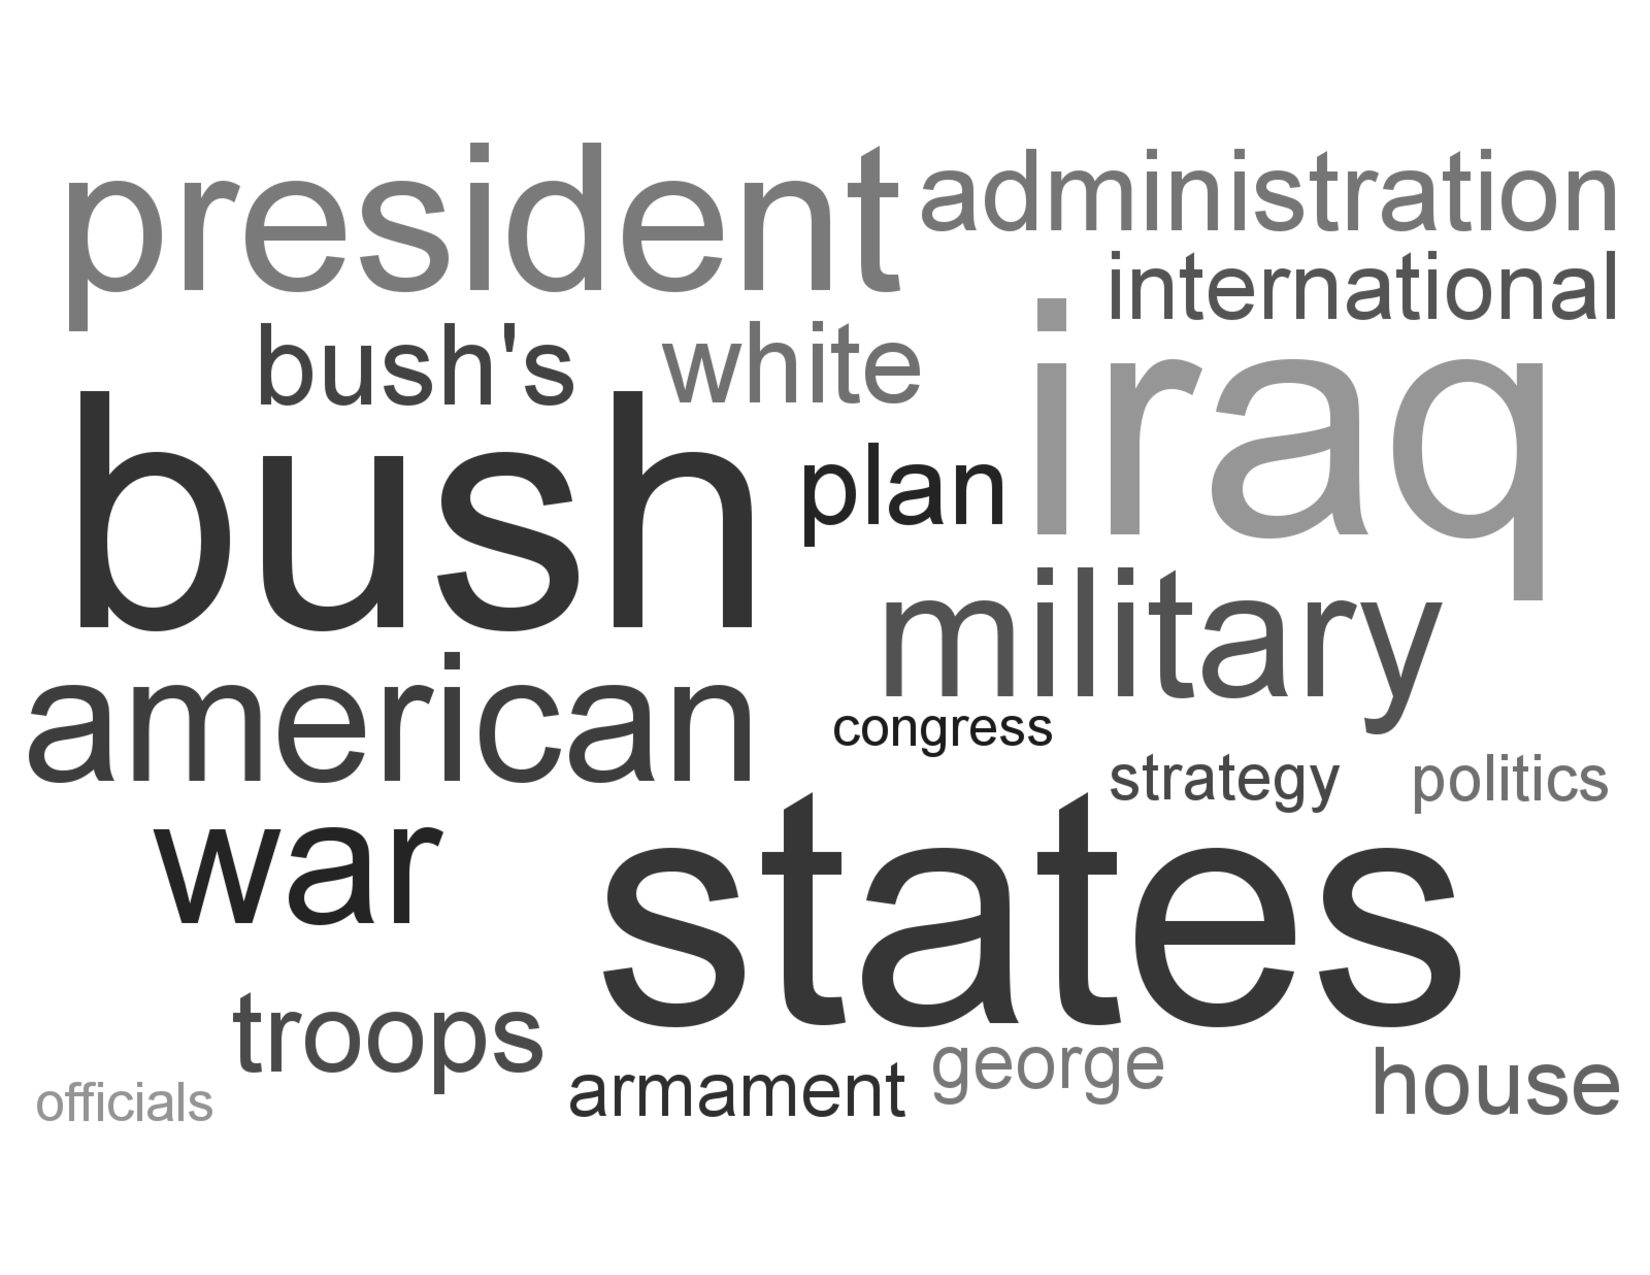
\includegraphics[width=.5\linewidth]{figures/wordcloud_20}
  \end{center}
  \caption{Word clouds use a 2D layout to show which words appear in a
  topic.  Word size is related to its probability in the topic,
  showing which words are more prominent.}
  \label{fig:word-cloud}
\end{figure}

Word clouds (e.g., Figure~\ref{fig:word-cloud}) are another popular approach for
displaying topics.  Unlike word lists, they also use the size of words to convey
additional information. Word clouds typically use the size of words to reflect
the probability of the words.  This uses more of a given visualization area to
be used to display a topic.

\begin{figure}
  \begin{center}
    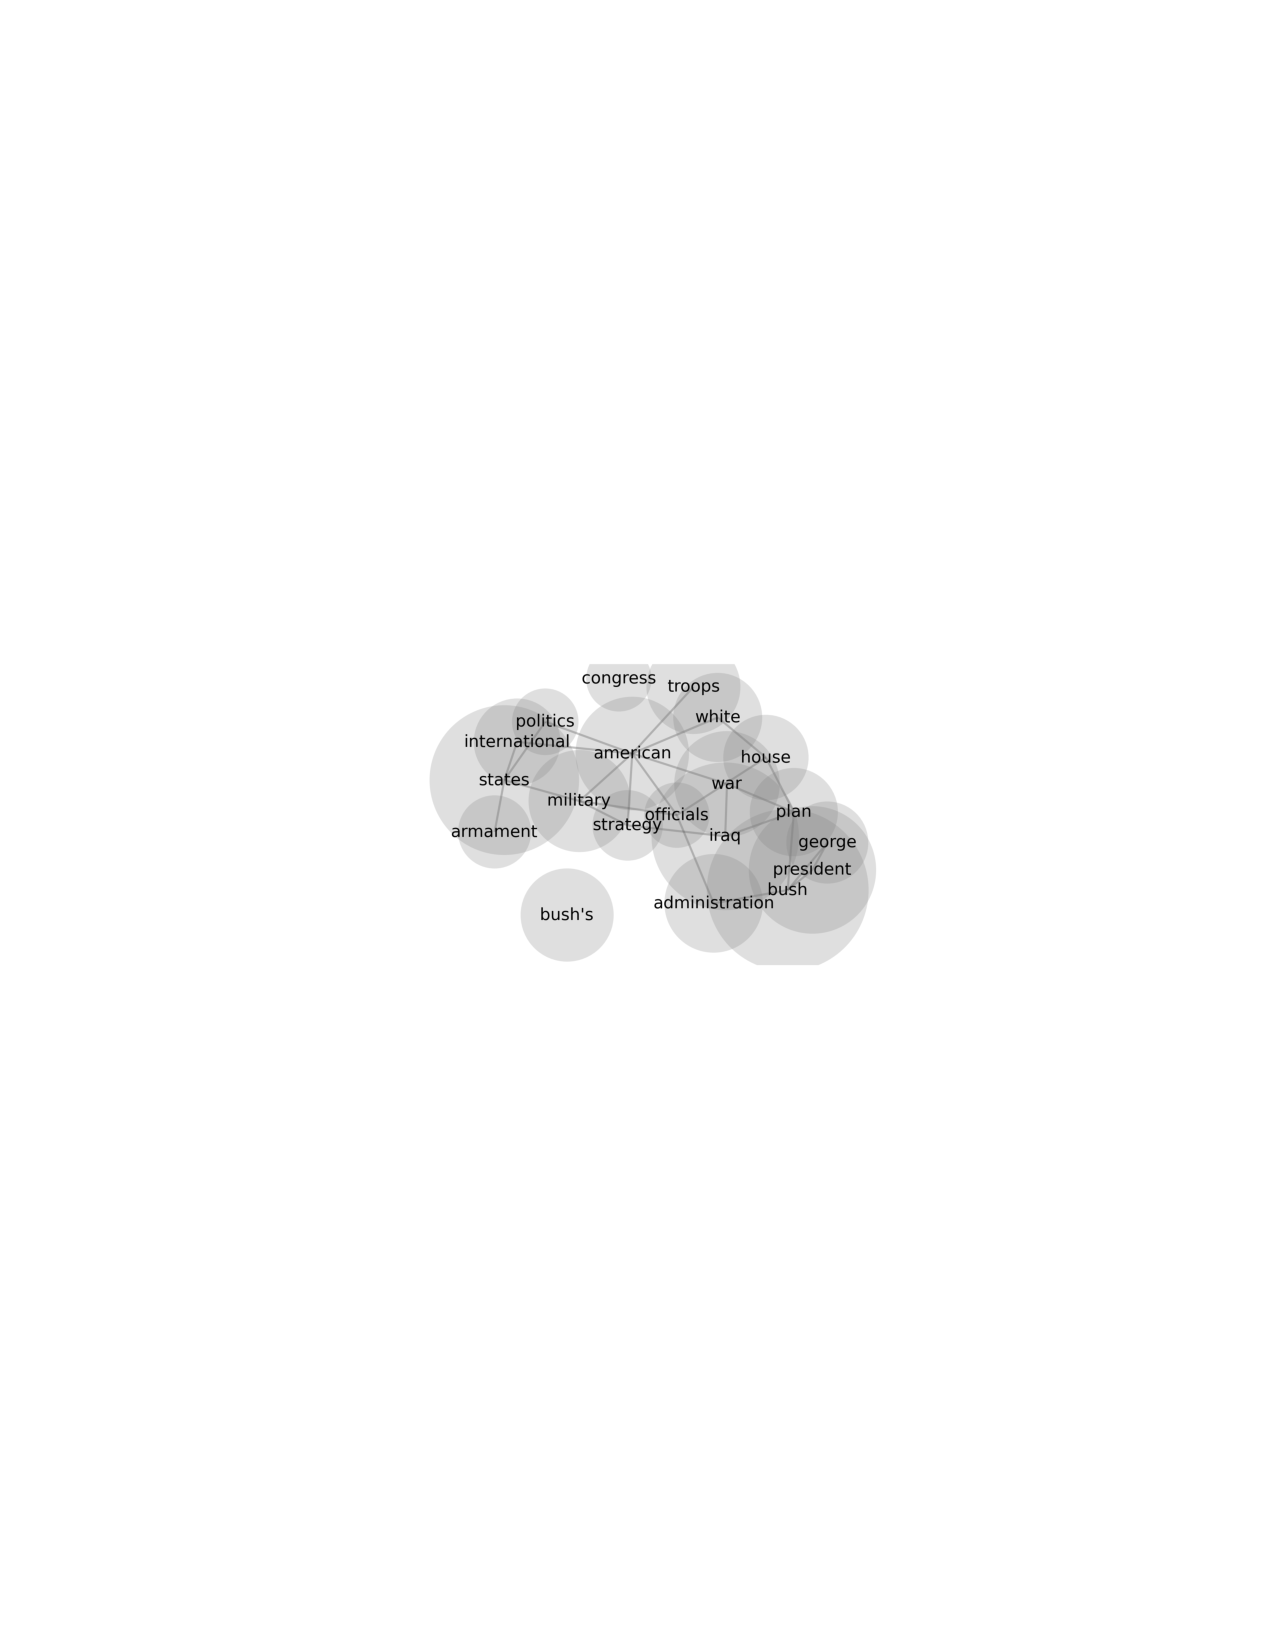
\includegraphics[width=.5\linewidth]{figures/topic_in_a_box_20}
  \end{center}
  \caption{A topic-in-a-box visualization for topics---like a word
    cloud---shows words in a 2D context.  However, it uses local
    co-occurence to decide which words to place next to each other.}
  \label{fig:topic-in-a-box}
\end{figure}

However, word clouds have been criticized for providing poor support for visual
search~\cite{Viegas2008} and lacking contextual information between
words~\cite{harris11}; users can sometimes draw false connections between words
that are placed next to each other randomly in a word cloud.  Another
alternative is to use word associations to layout
words~\citep{Smith:Chuang:Hu:Boyd-Graber:Findlater-2014};
Figure~\ref{fig:topic-in-a-box} shows places words that appear together next to
each other in the visualization.

% \subsection{When Words aren't Enough}

% Multi-word expressions can be discovered through
% pre-processing~\citep{talley-11}, post-processing step~\citep{blei-09b},
% or a joint model~\citep{johnson-10}.

\section{Labeling Topics}

Throughout this survey, we've been referring to topics about
\underline{information technology} or about \underline{the arts}.  These are
convenient labels, but completely removed from the raw distribution over words.
Thus, it's often useful to assign labels to topics within an interface.

In contrast to the previous \emph{visualization} approaches, labeling
focuses son showing not the original words of a topic but rather a
clearer label more akin to what a human summary of the data would
provide.

Approaches for automatic labeling can be divided into those that only
use internal information from the topic model against those that also
use external knowledge resources.  While purely internal methods are
more robust and consistent with the philosophy of unsupervised topic
models, external resources often produce higher quality
labels.

Of the techniques that use external resources, we further separate
those that use direct supervision for labeling (i.e., knowing what
constitutes a good labeling) from those that use general knowledge
resources such as Wikipedia or knowledge bases.

\paragraph{Internal Labeling}

\citet{mei-07} propose an internal labeling method that takes
prominent phrases from the topic and compares how consistent the
phrase's context is with the topic distribution.  Phrases whose
contexts closely resemble the topic often appear in regions of text
that summarize the document, making them good candidates for labels.
\citet{mao-12} extend the technique to hierarchies, using the insight
that parents' labels should be consistent with their children's.

% What about Tim W at UIUC?

% I didn't really understand this paper: Automatic Labelling of Topic
% Models Learned from Twitter by Summarisation (shoud we cite?)

\paragraph{Labeling with Supervised Labels}

% Frank Wood / Noemi hierarchically supervised model?

\citet{lau-10} use a supervised approach to rerank the words in a
topic to ensure that the ``best'' word in the topic is shown to a
user. Each candidate word forms a feature vector consisting of
features such as the following:
\begin{itemize*}
\item the conditional probability of a word given the other words in a
  topic (which implies topic coherence, as discussed in
  Section~\ref{sec:coherence});
\item whether the word is a hypernym of other words in the topic
  (e.g., ``dog'' in a topic that also contains ``terrier'' and
  ``poodle''); and
\item the original probability of the word in the topic.
\end{itemize*}

While these can be used alone as an unsupervised reranking,
\citet{lau-10} use user-selected best topic words to weight which of
these features are most important for selecting the best topic word.
These weights are learned using support vector regression.
\citet{lau-11} extend their technique by adding candidates from
Wikipedia to the set and show that models learned on different domain
corpora are still effective.

\paragraph{Labeling with Knowledge Bases}

% Perhaps have a figure to give an example
\citet{mao-12} align topic models with an external ontology of labels.
They argue that labels should match topic words (as labeling with flat
topics); a topic's words should be consistent with a labels' children
in the hierarchy; and the topic's labels should be unique.

\citet{aleteras-14} instead query the whole web and then build a graph that
includes the words that make up the titles of the retrieved webpages. The edges
between the words is the \abr{npmi} computed on a reference corpus.  The
intuition is that words that are ``central'' in this graph will be a good title
for the topic.  They find the central words by using the PageRank~\citep{page-99}
algorithm.  This finds words that are highly probable in the topic and appears
often with many other words in the topic.

\paragraph{Using Labeled Documents}

The task of associating labels with topics becomes much easier if many of your
documents are themselves labeled.  Labeled \abr{lda}~\citep{ramage-09}
associates topics to each of the labels and forces labeled documents to only use
the topics associated with the document.  This constraint forces the topics to
be consistent with the original labels (Figure~\ref{fig:llda}).
\citet{Bakalov-12} extend this to hierarchical label sets (e.g., \abr{ny} Times
subjects that place \underline{Russia} under \underline{International}), while
\citet{nguyen:boyd-graber:resnik:chang-2014} extend it to learning hierarchies
of topics from unorganized labels, learning that \underline{ska} topics are a
kind of \underline{music} without provided links.

\begin{figure}
  \begin{center}
    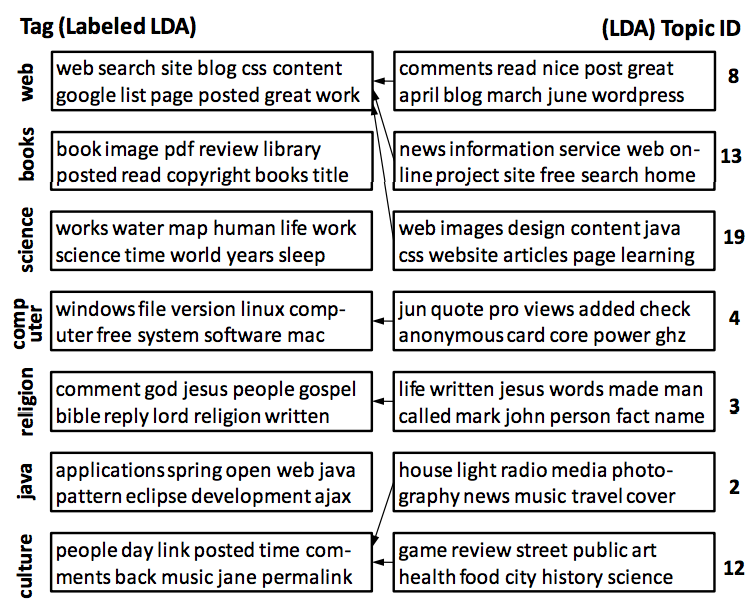
\includegraphics[width=.5\linewidth]{figures/viz_llda}
  \end{center}
  \caption{Example of topics learned by labeled \abr{lda} (Figure from
    \citet{ramage-09}).  Each topic in labeled \abr{lda} is associated with a
    label, which encourages the topics to be consistent with the ontology of
    labels.  \abr{lda}, in contrast, uses the empirical frequency of topics to
    divide the dataset, resulting in three topics (8, 13, 19) associated with
    the labeled \abr{lda} \underline{web} topic. }
  \label{fig:llda}
\end{figure}


\section{Displaying Models}

\begin{figure}
  \begin{center}
  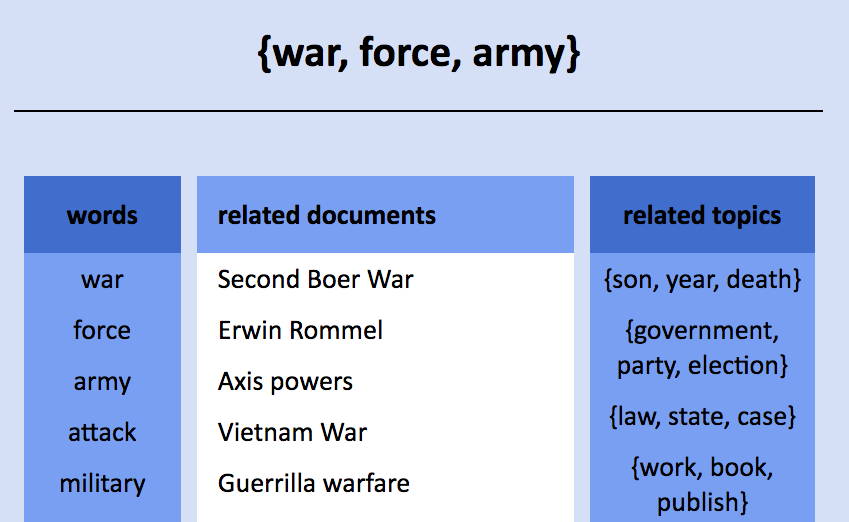
\includegraphics[width=.8\linewidth]{figures/viz_tmve}
  \end{center}
  \caption{The Topic Model Visualization Engine~\citep{chaney-12}
    shows the most related documents to a topic along with related topics. }
  \label{fig:tmve}
\end{figure}

However, topics are not the end of the story.  Users often want to use topics to
find relevant documents within the collection.  Going back to our example in the
previous chapter, a user may want to find the ``smoking gun'' in the Enron
dataset, not just use topics to understand the main themes in a dataset.

Thus, a good topic model visualization must also show the documents associated
with a topic.  The Topic Model Visualization Engine~\citep{chaney-12} shows the
top documents associated with a topic (Figure~\ref{fig:tmve}).  Recall that each
document has a distribution over topics $\theta_d$, which is a vector with an
entry for each topic.  We focus the dimension associated with a particular topic
and then sort the documents based on that topic coordinate from largest to
smallest.

The topical guide~\citep{gardner-10} extends this approach by enriching topic
views with additional metadata.  For instance, if the collection has dollar
amounts or sentiment~\cite{pang-08} associated with a document, it provides a
histogram of the metadata associated with the topic.  It also provides \emph{in
  context} examples of topic words, allowing to see how a word is used within a
topic (helping to address topic model's bag of words assumptions).

\abr{tome}~\citep{eistenstein-14} focuses on a specific type of metadata: time.
It allows users to view the evolution of topics over time to understand, for
example, how the issue of slavery is reframed from an economic argument to an
argument over human rights.  It supports filtering to specific topics or to see
how words are used over time across topics.

In contrast to showing how topics related to metadata,
\citet{chuang-12} focus on how topics relate to \emph{each other}.
Their ``Termite'' topic visualization (Figure~\ref{fig:termite}) shows
the term-by-term similarity between topics.  By presenting topic-term
probabilities on a grid with topics as the columns and terms as the
rows, users can see when topics share words or when topics are only
about a handful of words.

\begin{figure}
  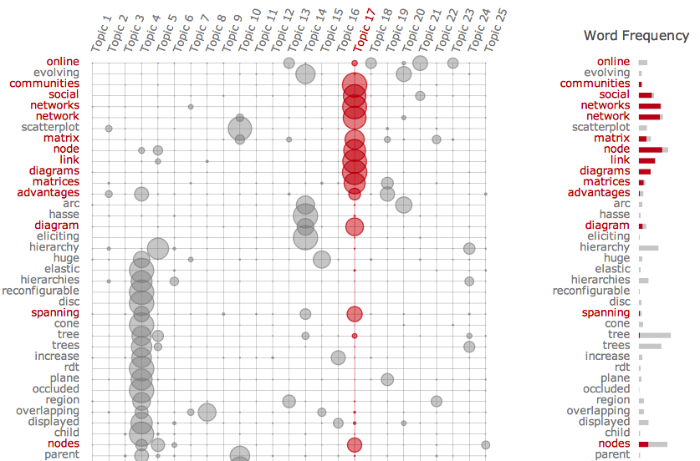
\includegraphics[width=.9\linewidth]{figures/viz_termite}
  \caption{The Termite visualization of topics helps reveal which
    topics use similar words and are thus likely talking about similar
    things.}
  \label{fig:termite}
\end{figure}

\section{Quality, Stability, and Repair}
\label{sec:coherence}

However, not all topic models are perfect.  \citet{chang-09b} showed that
held-out likelihood, the traditional measure of probabilistic model quality,
emphasizes \emph{complexity} rather than interpretability, what humans
presumably care about.  Thus, automated techniques may not be able to tell you
whether a topic model is good or not.\footnote{Automated
  measurements~\citep{newman-10,mimno-11,lau-14} of topic quality may serve as a
  proxy for human interpretability ratings.}

Visualizations can help show users where topic models have issues.
Showing the relationships between multiple models can also help
distinguish stable from spurious topics~\citep{chuang-15}, and
adjusting the ``hyperparameters'' of distributions (the Dirichlet
parameters of models discussed in Chapter~\ref{ch:intro}) can have a
large effect of what the final models are~\cite{wallach-09b}.

Interactive topic modeling---in conjunction with visualizations---can help
correct the problems of topic models.  A user first get an overview of the
dataset using a visualization of the topics and documents.  Then, the user can
see instances where the model errs and then correct those mistakes.

For example, Figure~\ref{fig:itm-nih} shows a topic learned from abstracts of
grants funded by the American National Institutes of Health
(\abr{nih}, discussed more in Chapter~\ref{sec:sci_fields}).  Most
topics were ``good''; they summarized the data and told a story about
a coherent slice of research supported by the \abr{nih}.  However,
this topic is more problematic; it combines words about the central
nervous system with words about the urinary system.  Such a topic (as
discussed in \citet{mimno-11}) does not give a clear understanding of the
documents it should represent.

\begin{figure}

\begin{minipage}[b]{0.4\textwidth}
\begin{tabular}{p{.9\textwidth}}
	Topic Words (before) \\ \hline \red{bladder}, sci,
        \blue{spinal\_cord}, \blue{spinal\_cord\_injury},
        \blue{spinal}, \red{urinary}, \red{urinary\_tract},
        \red{urothelial},\blue{injury}, \blue{motor}, \blue{recovery},
        \blue{reflex}, \blue{cervical}, \red{urothelium},
        \blue{functional\_recovery} \\
\end{tabular}
\end{minipage}
  \hfill
\begin{minipage}[b]{0.4\textwidth}
\begin{tabular}{p{.9\textwidth}}
	Topic Words (after) \\ \hline sci, \blue{spinal\_cord},
        \blue{spinal\_cord\_injury}, \blue{spinal}, \blue{injury},
        \blue{recovery}, \blue{motor}, \blue{reflex},
        \red{urothelial}, \green{injured},
        \blue{functional\_recovery}, \green{plasticity},
        \green{locomotor}, \blue{cervical}, \green{locomotion}\\
\end{tabular}
\end{minipage}

\caption{Before and after topics with iteractive topic modeling from
  \citet{hu-14:itm}.  Initially, this topic conflates two topics
  (\red{urinary} and \blue{central nervous system}), which is undesierable.  Adding
a constraint that the words ``bladder'' and ``spinal cord'' shouldn't
appear together in a topic makes the topic more coherent and discovers
concepts that \green{weren't present before}.}
\label{fig:itm-nih}
\end{figure}

\citet{hu-14:itm} address this problem by allowing a user to add probabilistic
constraints to the model~\citep{boyd-graber-07,andrzejewski-09}.  For example,
the user might say that ``bladder'' and ``spinal cord'' don't belong in the same
topic together.  Figure~\ref{fig:itm-nih} shows how the topic is more focused after the
user provides this feedback.  In contrast to probabilistic constraints,
\citet{choo-13} add matrix factorization constraints, which are in practice much
faster.

\section{Conclusion}

Much of what topic models are used for is to help users understand corpora.
However, the output of topic models don't give insights to users without the
helpmeet of interactive visualizations which allow users to discover and
refine insights.  In the next chapters we'll talk about specific applications of
these insights, but these insights are often built on the initial understanding
of a model offered by the visualizations discussed in this chapter.


\chapter{Historical Documents}
\label{ch:nonfiction}

Topic models play an important role in the analysis of historical documents.
Historical records tend to be extensive and difficult to manage without intense and time-consuming organization.
Records are complicated: they resist categorization, and may even lack standard spelling and formatting.
But there is more to history than simply the management of documents.
The task of a historian is not only to absorb the contents of historical records, but to generalize; to find patterns and regularities that are true to the documents, but also beyond any single piece of evidence.
Topic models are useful because they address these issues. They are scalable, robust to variability, and able to generalize while remaining grounded in observation.

Automated methods are an especially valuable counterpoint to traditional scholarly methods.
Studying history is about encountering the unexpected, often in contexts that seem familiar.
We don't necessarily know how people in the past talked about particular issues, or how they organized their lives.
Perhaps more dangerously, we assume that we know these things, and that our ancestors saw the world in the same way we do.
Topic models give us a perspective that is interpretable but at the same time alien, based on patterns in documents and not on our own conceptions of how things should be.

Time is a critical variable in the study of historical documents.
Although many modern collections have a significant aspect of time variation (see for example scientometrics), time is a defining element of historical research.
Collections of historical documents are necessarily situated in a time other than our own, but also tend to cover long periods---decades or even centuries.
As a result, many of the examples cited in this chapter organize documents along a temporal axis.
The associated analysis is particularly concerned with how language, as reflected in topic concentrations and topic contents, changes over time.

This chapter is organized around different formats for historical documents.
A recurring focus is the desire to plot events and discourses against time.
We begin with historical newspapers, which are relatively close to the modern news articles that are a more familiar use case in topic modeling.
We then consider other forms of historical records, such as annals and diaries.
These demonstrate the flexibility of topic modeling, including a corpus not in English and corpus in English with irregular spelling.
Finally, we consider studies of historical scholarly literature.

%A useful resource:
%Clay Templeton, Topic Modeling in the Humanities: An Overview.\footnote{http://mith.umd.edu/topic-modeling-in-the-humanities-an-overview/}

\section{Newspapers}

\index{newspaper}
\citet{newman-06} present an example of topic modeling on historical newspapers,\footnote{\citet{mei-05} present an earlier example of \emph{contemporary} news analysis (i.e., where the data are already digitized).  Their work also uses topic models to show the evolution of themes over time.} in a collection of articles from the {\em Pennsylvania Gazette} from 1728 to 1800.\footnote{http://www.accessible-archives.com/}
These articles comprise 25 million word tokens in articles and advertisements, and cover several generations of everyday life before, during, and after the founding of the United States of America.
The authors contrast their study to manually created keyword-based indexes, which focus on specific terms and can be applied inconsistently across large corpora.
Spurious patterns in index term use could complicate historical research.
They cite an example of the tag {\em adv}, which is used extensively in the early and late decades of the corpus, but not in the middle.
The topic-based approach is attractive because it is consistent across the collection (as long as the terms used in the documents are themselves consistent) and because it operates at a more abstract semantic level, reducing the chance that modern historians miss key terms.

They compare three methods for finding semantic dimensions, latent semantic analysis \citep{deerwester-90}, $k$-means clustering, and a topic model \citep{hofmann-99}.
The difference between these methods can be described in terms of expressivity.
\abr{lsa} is effective at embedding word types and documents in a low-dimensional space, but the individual dimensions of this space are not interpretable as themes.
\abr{lsa} is too expressive: it places no constraints, such as positivity, on the learned dimensions, and therefore produces uninterpretable results that nevertheless fit the document set well.
The k-means clustering is more similar to the topic model, and more successful at finding recognizable themes.
But it is also prone to repeating similar clusters with small variations.
Because of the single-membership assumption (a document can only belong to one cluster), the clustering model cannot represent documents with varying combinations of somewhat independent themes.
The k-means model is therefore insufficiently expressive: it it forced to ``waste'' clusters on frequent combinations of simpler themes.
The topic model, in contrast, has both modeling flexibility along with sufficient  constraints to support interpretable results.

The authors find that the learned topics are a good representation of dynamics in the corpus, although not always in a direct manner.
There is a large increase in discussions of politics in the period immediately around the American Revolution ({\em state government constitution law united power}).
There is also evidence of economic factors: a topic relating to descriptions of cloth ({\em silk cotton ditto white black linen}) rises in the 1750s, but then declines as Americans turned to domestic ``homespun'' cloth production in response to British trade policies.
Other topics point to more subtle changes in language.
A topic that is less immediately interpretable ({\em  say thing might think own did}) corresponds to a series of long ``public letters'' that contain more academic ``argument making''.  This is consistent with other results~\citep{viermetz-08} that suggest topics may be long-term or transient, which is captured directly by \citet{viermetz-08}.


Nelson studies topics in Civil War-era newspapers, including the Confederate paper of record, the Richmond Daily Dispatch.\footnote{Mining the Dispatch, http://dsl.richmond.edu/dispatch/}
Like Block and Newman, Nelson's goal is to organize the collection into themes and to measure the variation in prevalence of those themes over time.
The web interface highlights a temporal view of the collection as a series of topic-specific time series.
The mode of analysis is neither fully automated nor manual, but rather combines the two approaches.
Nelson manually labels the topics and groups them into larger categories such as ``slavery'', ``nationalism and patriotism'', ``soldiers'', and ``economy''.

He validates the model by comparing topics to a known and previously annotated category, the ``fugitive slave ads''.
These documents were pre-photographic descriptions of runaway slaves, and have a specific language consisting of aspects of personal appearance and possible locations where enslaved people might have  hidden.
He finds a near perfect correspondence between the prevalence over time of manually labeled fugitive slave ads and documents that have a high concentration of a specific topic, which places high probability on terms such as {\em reward, years,} and {\em color} (manual labels were not used  in training the model).
Nelson notes that few if any of these documents are assigned completely to this topic: he uses a cutoff of 21.5\% as a criterion.

Nelson's larger-scale groupings of topics pick out threads of discourse that may or may not be correlated over time.
The model identifies three topics that have similar temporal distribution, peaking at the beginning of the war in 1861 and largely disappearing afterwards.
These are related but distinct themes: anti-Northern sentiment expressed in poetic form, anti-Northern sentiment expressed in vitriolic prose, and discussion of secession.
All three form aspects of the same process, the rhetorical push for war.
Other related topics have slightly different temporal distributions.
Nelson groups six topics related to soldiers, and displays them in the order of their maximum concentration over time.
They move from ``military recruitment'' and ``orders to report'' to later topics related to ``deserters'', ``casualties'', and ``war prisoners.''
Again, these are related themes but rather than comprising a single event they trace the development of the increasingly dire military situation of the Confederacy.

\citet{yang-11-historical} model a collection of historical newspapers from Texas spanning from the end of the Civil War to the present day.
The goal is both exploratory, to find out about the interests of Texans through the 19th and 20th centuries, and {\em semi-exploratory}, to find out more about the history and context of specific, pre-specified themes such as cotton production.
In the topic model setting, semi-exploratory analysis starts by identifying one or more topics that seem to correspond to the theme of interest, and then using those topics as a axis of investigation into the corpus.
For example, a historian considered documents that exhibit topics related to cotton, and the topics that co-occur in those documents.
The study also led to more fully exploratory results.
A \underline{Battle of San Jacinto} topic, the final conflict in the Texas Revolution that led to separation from Mexico, appeared earlier than expected.
Further investigation suggested that the significance of the pivotal battle of San Jacinto was established much earlier than historians had previously anticipated.

The Texas newspaper study raises several interesting methodological issues relating to pre-processing and iterative modeling.
The authors put considerable work into dealing with the quality of digitization.
There are many factors that affect the quality of digitized historical newspapers, from the quality of the original printing to scanning, article segmentation, and optical character recognition (\abr{ocr}).
For this study extensive work was applied to automated spelling correction.
Another notable factor in this study is its prominent use of multiple topic models.
In many cases there is a tacit assumption that a single corpus should result in a single model, but in practice modeling is often iterative, and intimately bound to the development of pre-processing systems.
\citet{alsumait-08} iteratively refine their model with each segment of a news collection, while
\citet{yang-11-historical} train different models on different temporal slices of the corpus.
Although there is some advantage to maintaining a consistent topic space over time, dividing the corpus into separate sections has certain advantages.
In this case, historians were interested in the context of specific historic periods, such as the full run of a newspaper in one of several pivotal years, that are smaller than the full corpus but yet too large to be read easily.
The authors also describe an iterative workflow that involves comparing topic model output after each of several pre-processing steps.
Topic models are often effective at identifying consistent data-preparation errors, such as end-of-line hyphenation and consistent \abr{ocr} errors.

\section{Historical Records}

Other types of records besides newspapers are of interest, and present their own challenges.
In this section we consider two case studies, in which the simplicity of the bag-of-words document model is an asset because it allows for substantial variability in spelling and language, both in English and in other languages.

\index{German language}
\citet{erlin2017topic} search for work related to epistemology in a large corpus of English and German books.
They ``seed'' the models for each language with a small set of query words that the authors expect to be related to that subject.
This approach is closer to standard information retrieval than many other topic model applications, since the model is used both as a way of organizing the corpus and as a way of focusing attention on specific aspects.
Their use of a topic model differs from standard IR in that they are more deliberately open to related terms and concepts: the field of epistemology is expected to be broad, and more likely to be represented by a combination of words than by any one query.

\index{Chinese language}
\citet{miller-13} uses Chinese records to investigate the meaning of
the word {\em zei}, or ``bandit'' in Qing dynasty China (1644--1912). The word by
itself can imply several different forms of anti-social behavior,
which are difficult to distinguish from word frequencies alone. A
topic model uses contextual information to separate these effects.

The application of topic models in Chinese highlights the importance of tokenization.
We usually receive documents in the form of long strings, but we are interested in identifying {\em tokens} that are short strings with a specific meaning.
Breaking a document into distinct tokens is an often-overlooked part of the document analysis process.
In European languages we can achieve good results simply by separating strings of letter characters from sequences of non-letter characters, although there are many special cases~\citep{Boyd-Graber-14}.
Tokens may contain non-letter characters such as apostrophes and hyphens, and may span multiple words ({\em Queen Victoria}, {\em black hole}).
In many East Asian writing systems we cannot rely on orthographic conventions to identify tokens.
Miller argues that in Classical Chinese a single character can be treated as a token without a strong negative impact on modeling, but for Japanese and modern Chinese we must often rely on pre-processing tools that are themselves potentially unreliable.

%\jbgcomment{Could we get a figure for the months?  I think that would be a nice addition}

\index{Martha Ballard}
Cameron Blevins models the diary of Martha Ballard (1735--1812), a revolutionary war-era midwife who recorded entries over 27 years.\footnote{http://www.cameronblevins.org/posts/topic-modeling-martha-ballards-diary/} The model provides a useful way to discover connections between words and repeated discourses.
As with other historical corpora, Blevins focuses on the connection between topics and time.
Specific events, like a birth, can be highlighted by looking at spikes in a certain topic in the day-to-day time series.
But larger trends are also evident.
As a calibration experiment, Blevins measures the association of a topic that appears to refer to cold weather ({\em cold, windy, chilly, snowy, air}) to months of the year.
As expected, the concentration of this topic is lowest from May to August, rises from September to January, and falls from February to April.

Blevins identifies several other topics that appear to change in their concentration over time.
Two topics involving house work, focusing roughly on cleaning and cooking, respectively, appear to be correlated in time, and rise over the decades.
Blevins connects this finding to suggestions that as Ballard grew older and her children moved away, she had less help from family members.
A more subtle topic involves descriptions of fatigue and illness.
This topic also increases over time, and appears to correlate with the housework topics, except in the last year of the diary, where fatigue and illness reach their highest concentration and housework declines.

This analysis exemplifies the exploratory nature of topic modeling: by themselves, these observations are not conclusive, but they are suggestive and point to areas of further analysis.
A scholar might take the diary entries that score high on an individual topic as a reading list, and determine how well a particular automatically detected discourse maps to themes in Ballard's personal experience.
For example, one might check whether Ballard's references to fatigue and illness are referring to herself or to patients.
The model does not tell the whole story, but it points to where stories might lie.

Blevins argues that characteristics of the diary form make it well-suited for topic analysis: ``Short, content-driven entries that usually touch upon a limited number of topics appear to produce remarkably cohesive and accurate topics.''
In addition, the topic model's lack of linguistic sophistication is actually an asset in this case.
The diary is written in a terse style with many abbreviations and with irregular, 18\textsuperscript{th} century spelling: ``mrss Pages illness Came on at Evng and Shee was Deliverd at 11h of a Son which waid 12 lb.''
Models trained on modern text corpora might not even recognize this example as English, but the topic modeling algorithm is still capable of finding semantically meaningful groups of words.



\section{Scholarly Literature}
\label{sec:scholarly}

%\jbgcomment{The definition of secondary literature seems unclear to me, and it's not clear that the problem of copyright has been discussed enough that it's clear that JSTOR is so great as a result (even though it is!)}

\index{\abr{jstor}}
The historical record of scholarship is a valuable source for intellectual history.
Many users make use of the \abr{jstor} ``Data for Research'' \abr{api}.\footnote{http://dfr.jstor.org/}
The \abr{dfr api} is an important example, because it provides access to articles that have been scanned by \abr{jstor} and may be under copyright.
Access to the underlying documents in their original form as readable sequences of words may be restricted for legal or commercial reasons.
\abr{dfr} provides a simple view into selected articles by only providing the frequency of word unigrams.
While the bag-of-words assumption used by topic models is restrictive, in this case it can be an advantage, because the original sequence of words is not used for inference anyway.

\index{German language}
\citet{mimno-12b} studies a collection of Classics journals digitized by \abr{jstor} to detect changes in the field over the 20\textsuperscript{th} century.
A distinctive aspect of this study is the use of a {\em polylingual} topic model~\citep{mimno-09}.  The details of this model and how it contrasts with other models are described in more detail in Chapter~\ref{sec:doc-align}; for this discussion we simply need some topic model that can discover topics that are consistent across languages.
An English-language journal is compared to a German-language journal by learning a common set of topics that each have a vocabulary in both languages.
In other words, a topic has two ``modes'', one in which it emits words drawn from a distribution over English terms, and another in which it emits words drawn from a distribution over German terms.
The linkage between English and German words is constructed using Wikipedia articles.
Wikipedia articles exist in many different languages, and articles in one language often link to comparable articles in another language.
The author first selects English Wikipedia articles matching key terms in the English-language journals, and then collects the German Wikipedia articles that are listed as being comparable to the selected English-language articles.

By training the topic model jointly on the combined corpus of the original journal articles and the comparable Wikipedia articles, the model provides insight into the relative concentration of scholarly interests across the two language communities.
The German-language journal articles contain relatively more work on law and oratory, themes that are present in the English-language articles but less prevalent.
The model also shows a large increase in  interest in poetry in the German journal in the period following the second world war.
In the English journals there is a large increase starting in the 1980s in cultural and economic studies along with critical theory, which does not appear in the German journals.

\citet{riddell-12} also approaches German scholarly literature from the 20\textsuperscript{th} century. He finds that topics align well with authors such as Goethe and subjects such as folklore. Apparent spikes in the use of these topics appear to align with anniversaries of authors (G\"othe, the Grimm brothers).
Riddell emphasizes that models are useful in raising issues but not a substitute for scholarship.
He comments that ``it becomes essential that those using topic models validate the description provided by a topic model by reference to something other than the topic model itself.''

\citet{Goldstone-14} use a topic model as a tool to structure an exploration of a corpus that spans more than a century.
They are interested both in changes at the topic level and at the level of word use within topics.
For these authors the appeal of topic modeling is that models are better able to represent contextual meaning than simple lists of keywords. They write that ``[t]he meanings
of words are shifting and context-dependent. For this reason, it is risky to
construct groups of words that we imagine are equivalent to some predetermined
concept.''

\index{Modern Language Association}
They analyze the proceedings of the Modern Language Association\footnote{The MLA is a professional organization for literary scholars in the United States.} to find shifts in focus in the field of English literature.
A model trained with 150 topics on 21,000 articles identifies a topic associated with descriptions of \underline{violence}: {\em power,
violence, fear, blood, death, murder, act, guilt}. Using a temporal plot they argue that the concentration of this topic is greater in the second half of the 20\textsuperscript{th} century than during the first half.
They contextualize this finding by comparing the frequency of these words in a more general corpus from Google n-grams; there is no comparable change.
This approach holds the topic fixed and searches for associated words.
They then pivot and hold the word ``power'' fixed and search for associated topics.
In this case the \underline{violence} topic actually appears to be relatively stable in its association with the target word. The largest increase is in a different topic characterized by the words {\em own power text form}, in which context it appears almost exclusively after 1980.
Like many topics, the content of this topic is difficult to assess from top words alone.
Further exploration through exploration of individual documents would be necessary (e.g., through the tools discussed in Chapter~\ref{ch:viz}).

\section{Summary}

This chapter focuses on finding themes in document that reflect temporal trends.
When we consider newspapers, historical records, and historical scholarly journals we are looking not just for the topical foci of each time period, but how those topics shift in concentration as they are influenced by historical events.
Modeling large collections of documents allows us to reveal how events are reflected in writing and how ideas and emotions emerge in response to changing events.

In the next chapter, we extend our discussion of scholarly journals to focus more directly on how new ideas emerge.
Unlike newspapers and diaries which reflect the reality of the world, the writing in scientific manuscripts can actually change the world by introducing innovative technologies.
The next chapter asks whether we can detect and describe these innovations.


\chapter{Fiction and Literature}

\label{ch:fiction}

This chapter considers documents that are valued not just for their information content but for their artistic expression.
There are many different ways to read fiction, poetry, and rhetoric, and the choice of how we read affects the type of conclusions that we are able to make.
Scholars have traditionally focused on a ``close reading'' approach, in which the goal is to identify the specific features of a passage that convey a more general meaning, or emotion, or atmosphere.
These features might include nuances of word  selection, echoes of sound through rhyme or alliteration, or prosodic features like rhythm or cadence.

\section{The Role Topic Models Play in the Humanities}

While close reading is a foundational tool in the study of literature, it is necessarily limited by its scale.
We value literature because it is one of the best ways to capture the spirit of an age, and the experiences of those who lived through it. But standard close reading methods require narrow focus and thorough interpretation.
Topic models complement close reading in two ways, as a survey method and as a means for tracing and comparing large-scale patterns.

The survey method is relatively simple, linking passages that a reader may not have known about.
Close reading is the best way to analyze a short passage of text, but which short passages of text do we want to analyze?
Because no one can read --- much less close read --- all the available material from a culture or time period, scholars are often left trying to make large-scale arguments about the history of literature from small-scale evidence. And this small-scale exploration is not randomly selected: the same small canon is studied in detail while the vast proportion make up the ``great unread'' \citep{moretti-00}, works that are never studied.
Identifying broad themes and then mapping those themes to their realization in different contexts may reveal works or sections of works that are ``hiding in plain sight,'' unknown to modern scholarship simply through obscurity.

An alternative, and less traditional, mode of analysis is often referred to as ``distant reading'' \citep{moretti-13}.   This approach uses computer-assisted methodologies. Topic modeling has emerged as a central tool in distant reading, as a way to organize our reading of large scale patterns.

Topic analysis, viewed as a way of identifying repetitions of language or discourse through multiple works, resonates with many more familiar approaches to the study of literature.
At the broadest scale, to define a genre or a literary period is to separate a corpus into sections based on some observable criterion.
We posit a ``gothic'' literature characterized by atmospheric descriptions of castles, or a ``cyberpunk'' literature characterized by conflicted relationships with information technology.
At a smaller scale, themes or tropes reappear in different contexts.
At the most detailed level, scholars identify repeated phrases, such as the descriptive epithets used in Homeric oral poetry.

Statistical topic analysis has a similar goal, but pursues it through different means.
Rather than rigid boundaries specified by date of publication or nationality, algorithms identify genre through the repeated words that form the traces of those themes.
Topics do not represent themes themselves, but rather identify the implicit statistical regularities in word use brought about by the presence of genres, themes, and discourses.


Applying topic models to fiction, however, brings new challenges.  \cite{jockers-13} trains a 500-topic model on a corpus of 4000 English-language novels.
Several issues emerge from this corpus. These are present in other contexts, but they are much more readily apparent in fiction.

\section{What is a Document?}

In most literature about topic models, the term ``document'' is used on the implicit assumption that users have things called documents.
In the canonical LDA article \cite{blei-03}, this word is used 143 times, but never defined.
In many cases, the meaning of a ``document'' is fairly clear: a news article, or a scientific abstract.
What was not clear in this earlier work was that this definition can be problematic, especially for documents longer than a few pages of text.

Treating novels as a single bag of words, for example, does not work.
Topics resulting from this corpus treatment are overly vague and lack thematic coherence.
We should not be surprised by this finding.
The assumption of a topic model is that the concentration of topics over a document is fixed and unchanging from the beginning of a document to the end.
Natural writing rarely fits the topic model assumption, and a novel that had no thematic variation over its entire length is unlikely to have been published.

We need to find a good segmentation into shorter contexts.
We assume that themes are expressed in different sections of a long document like a novel.
If a segmentation does a good job of identifying the boundaries between these sections, each resulting segment should have relatively few themes.
If a segmentation does not do a good job of identifying boundaries, we should see segments that contain more themes on average, because our segments combine fragments of multiple thematic segments.

 \cite{jockers-13} chooses to avoid relying on structural markers such as chapter divisions and divides novels into 1000-word chunks.
This treatment results in coherent, tightly focused topics that can be reasonably used as proxies for recognizable themes.

Although fixed-length segmentation is effective, it is not necessarily ideal.
\cite{algeehewitt2015paragraphs} compare varying fixed-length segmentations to segmentation based on paragraphs.
They evaluate the difference between treatments by measuring the concentration of topics in each segment of text after modeling.
The Herfindahl index is a measure of concentration in discrete probability distributions, calculated as the sum of the squared probabilities of each possible value:
\begin{align}
\text{Herfindahl}(P) = \sum_x P(x)^2.
\end{align}
For example, consider two distributions $P$ and $Q$ over a set of symbols $\{a, b, c, d, e\}$.
If $P$ has non-zero probability only on a single symbol $P(a) = 1.0$ and zero probability for all other symbols, the Herfindahl index of $P$ will be 1.0.
If $Q$ has uniform probability on all five symbols $Q(a) = Q(b) = ... = Q(e) = 0.2$, the Herfindahl index will be $5 \cdot \frac{1}{5} \cdot \frac{1}{5} = 0.2$.

When a corpus of 19th-century novels is divided by paragraphs, the Herfindahl index over concentration of topics within each segment is consistently larger than the same index calculated when the same corpus is divided into evenly sized 200-word slices, implying that the distribution over topics for each segment is more focused on a smaller number of topics.
Setting the slice size to the average length of paragraphs in the corpus, 82 words, increases the Herfindahl concentration metric, but the resulting value is still smaller than the value based on paragraphs.
This result is reassuring, in that it suggests that paragraphs do indeed have some consistent meaning, at least in this collection of 19th-century novels.

%\jbgcomment{We've not talked about twitter anywhere else, I think it would be a good example here}

% Comparison with Twitter?

\section{People and Places}

Because most works of fiction are set in imaginary worlds that have no existence outside the work itself, they are often characterized by words such as character names that are extremely frequent locally but never occur elsewhere.
This word co-occurrence pattern is problematic for topic models because they can be thought of as machines for finding groups of words that occur frequently together and not in other contexts.
Character names are --- by that criterion --- a perfect topic.
Modeling these documents can result in topics that are essentially lists of character names.

As an example, consider a model of 14 novels by Charles Dickens.
The top 20 words from a selection of topics ($K=50$) are shown in Table \ref{tbl:dickens-with-names}.
Upper-case letters are not reduced to lower-case in order to emphasize the presence of proper names.
Several topics are dominated by capitalized names, with individual novels clearly identifiable: Topic 4 is {\em Oliver Twist}, Topic 5 is {\em Nicholas Nickleby}, Topic 6 is {\em The Pickwick Papers} and Topic 7 is {\em A Tale of Two Cities}.
In fact, exactly half of the distinct words in the top 20 words for all topics are capitalized, and almost all of these are proper names.

Focusing on characters is not always uninformative, and can in some cases highlight structure within works.
Topics 1--3 all refer primarily to {\em Bleak House} (with the exception of {\em Scrooge}), but focus on different interlocking subplots.
The first focuses on Lady Dedlock, the second on Mr. Jarndyce and his two wards, Richard and Ada, and the third on the investigations of the detective Mr. Bucket.
The plot centers around the revelation of the connections between these apparently unrelated groups.

\begin{table}[htp]
\caption{Sample topics from Charles Dickens novels, without removal of character names (ordered manually).}
\begin{center}
\begin{tabular}{|c|p{15cm}|}
1 & Lady Leicester Scrooge Dedlock Rouncewell ladyship Wold Chesney Ghost Volumnia Christmas Tulkinghorn family Spirit Baronet nephew Rosa Scrooge's housekeeper Lady's \\
2 & Richard Jarndyce guardian Ada Charley Caddy dear Skimpole Miss Summerson Esther Jellyby miss Vholes Kenge Woodcourt quite myself Guppy Chancery \\
3 & says George Bucket Snagsby Guppy returns Smallweed Bagnet comes Tulkinghorn looks takes trooper does makes friend goes asks cries Chadband \\
4 & Oliver replied Bumble Sikes Jew Fagin boy girl Rose Brownlow dear gentleman Monks Noah doctor Giles Dodger lady Nancy Bill \\
5& Nicholas Nickleby Ralph Kate Newman replied Tim Mulberry Mantalini Creevy brother N oggs Madame Gride Linkinwater Smike Arthur rejoined Wititterly Ned \\
6 & Pickwick Winkle replied Tupman Wardle gentleman Snodgrass Pickwick's Perker fat boy Bardell dear Jingle inquired Fogg Dodson friends friend lady  \\
7 &  Lorry Defarge Doctor Manette Pross Carton Darnay Madame Lucie Monseigneur Cruncher Jerry Stryver prisoner Charles Monsieur Tellson's Marquis father Paris \\
8 & coach uncle gentleman lady box coachman gentlemen landlord get London guard inside horses waiter boys mail passengers large better hat \\
9 & street door streets windows houses room window few iron walls wall rooms dark within shop doors corner small stood large  \\
10 & money letter paper business read pounds papers five hundred office thousand clerk paid years pen next law desk letters week \\
\end{tabular}
\end{center}
\label{tbl:dickens-with-names}
\end{table}%


\cite{jockers-13} approaches this problem by constructing a stopword list that removes all character names before modeling.
There are many ways to construct such lists.
Lists of common names are a good start, but may not be aligned with a specific corpus.
Some languages mark proper names with orthographic conventions like capitalization, but these tend to be noisy.
A useful heuristic in English is to identify terms that appear capitalized in more than 90\% of instances.
Even then, names that are also common words, such as {\em daisy} and the aforementioned Mr. Bucket, or words that appear capitalized for other reasons, such as {\em god}, may lead to unintended results.
Furthermore, some languages do not differentiate letter cases (Hebrew, Korean) and others use it for other purposes (all nouns in German).
Named-entity recognition tools scan text for patterns of language that indicate personal names, and may result in greater precision than simpler methods.
Nevertheless, there is no known way to avoid careful consideration of the meaning of words in context.

Novels describe people and places, but they are also created by people (authors) who are influenced by their cultural setting.
\cite{jockers-13b} perform a post-hoc analysis on Jockers' earlier 500-topic model to determine whether there is a connection between the use of specific topics and metadata variables such as author gender, author nationality, and year of publication.
They find that the concentration of many topics is strongly correlated with author gender, and that these correlations are statistically significant.
Such significance testing can be carried out by randomization and bootstrap tests.
Both methods create ``fake'' corpora that are similar to the real corpus but different in specific ways.
Randomization or permutation tests randomly shuffle the assignment of labels (such as author gender). If an observed correlation between a topic and an external variable is within the range of the correlations generated by randomly assigning documents to labels, there is little statistical evidence that that observed correlation is meaningful.
Bootstrap tests preserve the relationship between documents and metadata variables, but resample documents with replacement.
This test indicates whether a result depends on the presence or absence of a specific document.
If there is wide variation between randomly generated corpora, the observed correlation may be the result of unusual outliers rather than a consistent pattern.

While the use of statistical hypothesis testing methods is potentially valuable in the context of large-scale distant reading, a literary analysis is not --- and should not be --- like a clinical trial.
It is important to note some differences between their use in a scholarly context and their use in more typical scientific studies.
First, the presence of unusual outliers or singular examples can in fact be a positive result.
The suggestion that a particularly work may be radically different from supposedly similar examples could be the beginning of a new perspective.
At the very least, it can identify editing and curation issues.
Second, a critical variable in an analysis of statistical significance is sample size.
Unlike a designed experiment, this sample size is usually not within our control: we have the literature that we have.
Finally, it is vitally important to avoid the impulse to treat a significance score as a binary valid/invalid result.
If numeric scores should be used at all, they should be presented as a ``level of support'' given the documents that are available.
Humanists may also be fundamentally more comfortable with dubious hypotheses: an observed association with a 10\% chance of being purely random could still be a very strong result.

As an example, \cite{jockers-13b} evaluate an intriguing hypothesis, that a topic about religious foundations ({\em Convents and Abbeys}) is used more by unknown authors\footnote{Authors unknown to modern scholarship, not authors publishing under known pseudonyms.} than by either (known) male or female authors.
The conjecture is authors were choosing to remain anonymous in order to write about politically and religiously touchy subjects.
This correlation, however, showed large variability under a bootstrap test, and indeed one of the supposedly anonymous works turned out to be an abridgment of an Anne Radcliffe novel.
The pattern is still present without the effect of these works, but there is not a clear and undeniable association between anonymity and the questioning of religious authority.

In some cases fiction is set in the context of real places.
\cite{tangherlini-13} look at nested models of sub-corpora within Danish literature in a way that highlights connections between real-world events and cultural movements and fictional echoes.
Their method, which they describe as a topical ``trawl line,'' uses a user-specified sub-corpus as a query and then searches the remainder of the corpus for works that match to that query.
As examples, they find works influenced by the translation of Charles Darwin into Danish, works influenced by the ``Modern Breakthrough'', and works influenced by folklore and regional literature.


\section{Beyond the Literal}

One of the hallmarks of fiction and literature is the use of figurative language.
It is not obvious that unintelligent machines with no cultural understanding would have any ability to process such metaphors. However, \cite{rhody-12} demonstrates on a corpus of poetry that although topics do not represent symbolic meanings, they are a good way of detecting the concrete language associated with repeated metaphors.

Specifically, Rhody explores a corpus of 4500 poems that describe works of art (or {\em ekphrastic} poems).
She trains a 60-topic model, and highlights several particularly interesting topics.
One of these topics places high probability on {\em night, light, moon, stars, day, dark, sun, sleep, sky, wind, time, eyes, star, darkness, bright}.
The apparent meaning of the topic is clear, and well summarized by the single top word: night.
But Rhody finds that when she explores the {\em context} of this topic, the poems are all using a consistent metaphor relating night and sleep to death.
The concept of death does not appear in the top words --- poets are not addressing the issue directly.
Nevertheless, the model has identified an example of non-literal, figurative language even though, because it is grounded in the actual words, it has no ability to represent what the poets actually mean.
The model is able to do this because the poets are using a consistent ``surface'' language to represent a consistent metaphor.
The metaphor is not detectable directly, but a poet's use of a metaphor has a signature that is observable.

Rhody highlights a second topic that provides an example of a different type of non-literal meaning.
This topic places high probability on {\em death, life, heart, dead, long, world, blood, earth, man, soul, men, face, day, pain, die}.
Unlike the previous topic, the topic directly references death and life, but it also lacks what Rhody calls the ``unambiguous comprehensibility'' of the {\em night} topic.
But examining the context of poems that contain the topic reveals a different pattern.
These poems have a consistent {\em form} that Rhody describes as elegiac.
She writes that ``Paul Laurence Dunbar's 'We Wear the Mask' never once mentions the word 'death,' the discourse Dunbar draws from to describe the erasure of identity and the shackles of racial injustice are identified by the model as drawing heavily from language associated with death, loss, and internal turmoil --- language which 'The Starry Night' indisputably also draws from.''

\section{Comparison to Stylometric Analysis}

In addition to discussing what researchers have done in literary analysis with topic models, it is useful to consider how other technologies have been used in the same setting.
One of the most established applications of computation in the study of literature is stylometry, or more specifically the question of authorship attribution \citep{juola2006authorship}.
It is illustrative to contrast the goals and methods of stylometry with those of topic modeling.

The critical insight of modern stylometry is that it is easy for authors to shift the focus of their work, but much more difficult to alter the semi-conscious style of their language \citep{mosteller1964inference}.
The implication is that content-bearing words, such as nouns and adjectives, are a relatively poor indicator of authorship or at least authorial style, while functional words, such as determiners, conjunctions, and prepositions, carry more information about authorship.
Therefore, measures such as Burrows' delta \citep{burrows2002delta} restrict attention to the most frequent words in a corpus.

The contrast to topic modeling is clear: stylometric analysis focuses on frequent, low-information words and ignores content-bearing words, while topic modeling generally does the exact opposite.
We generally remove high frequency words using a stop list, and in fiction go even further in removing words that are overly distinctive of a particular work.
An assumption of topic modeling is therefore that the goal is to find thematic components that are {\em not} specific to one author, but rather exhibit themselves, with more or less variation, across multiple works.
Where stylometry seeks to see past what authors are saying and focus on how they are saying it, a use of topic modeling is to find instances where different authors are writing about the same thing.

\section{Operationalizing ``Theme''}

The use of topic modeling in the study of literature has been beneficial both for humanities scholars and for machine learning researchers.
For scholars, these models offer the possibility of a more precise approach to concepts that have traditionally been vague and impressionistic, such as theme, genre, and motif.
At the same time, and somewhat paradoxically, literary documents present such a radically different mode of language than news articles or scientific publications that they lead us to question the apparent precision of statistical approaches.

Topic models provide a way of operationalizing the concept of distant reading.
\cite{moretti2013operationalizing} defines this term as ``Taking a concept, and transforming it into a series of operations.''
He attributes this definition to \cite{bridgman1927logic},  who introduces the term in the context of measurement in physics: ``To find the length of an object, we have to perform certain physical operations. The concept of length is therefore fixed when the operations by which length is measured are fixed: that is, the concept of length involves as much as and nothing more than the set of operations by which length is determined.''
While topic models are an imperfect tool for measuring theme in literature, they do provide a much more powerful approximation of theme than anything that we have had previously.

But applying statistical models to literature also brings forward a series of challenges that highlight the amount of human interpretive work that must go into successful topic modeling.
Literary documents are of varied lengths, describe self-contained imaginary worlds, and are suffused with symbolic language.
We can address these issues through corpus curation and through interpretive reading of models, but in doing so we must necessarily confront the fact that we are not simply applying Bridgman's fixed set of operations.

\section{Summary}

Just as topic models provide a methodology for analyzing the creative, diverse \oe{}vre of authors and the emotions and thoughts of fictional characters, topic models can also help us build insights of real people.
Thanks to social media, we have a wealth of information about people sharing their thoughts and views online.  Topic models can help us use these data to better capture emotion,
beliefs, and relationships.  The next chapter discusses how topic models can
understand these messy, interesting properties of text.



\chapter{Understanding Scientific Publications}
\label{ch:sci}

Understaning scientific publications is important for funding
agencies, lawmakers, and the public.

Rigid classifications are difficult because fields
change~\citep{szostak-04}.

\section{Understanding Fields of Studies}

Topics can correspond to rough fields of studies.  This insight was
noted early in the development of topic models~\citep{griffiths-04}.

Topic models can show where official designations or labels conflict
with reality~\citep{talley-11}.

Where we have labels we trust, we can use them to constrain
topics~\citep{ramage-09}.

But if the labels are two coarse, we can use topic models to refine
them or organize the\citep{Nguyen:Boyd-Graber:Resnik:Chang-2014}

\section{How Fields Change over Time}
\label{sec:science_fields}

One way that science is unique from the fields discussed in the
previous chapters is that it is part of a continuous dialog.  Each
paper in its own way stands on the shoulders of giants. Topic models
for science thus need to be aware of the connections between documents
over time.

One of the first techniques to do this viewed topics as subtly
changing each year~\citep{blei-06b}.  Example of physics going from
ether to accelerators.

The flipping of a calendar page does not rule science, however;
changes can happen at any time~\citep{wang-06,wang-08}.

\section{Innovation}

Fields change because innovation happens.  Identifying who is
responsible for the changes can find who is ``winning'' the race to
introduce, explain, and popularize new ideas.

From an institutional perspective, we can see which universities have
research portfolios that look like the future~\citep{ramage-10}.

This is important not just for science historians but also for policy
makers~\citep{largent-12}.

Institutions are where science happens, but the true drivers of
innovation are individual researchers who present their papers as the
place where research happens~\citep{gerrish-10}.


\chapter{Computational Social Science (jordan)}
\label{ch:css}

 while the previous chapters were mostly retrospective analyses, computational social science is mostly in the "here and now".

 traditional social science methods like polling do not scale well. And still require a lot of resources and time.

\section{Sentiment Analysis}

\section{Understanding Stance}

\section{Predicting Polarization}

\section{Discovering Framing}

Introduce hierarchies here



%\chapter{Multilingual Data and Machine Translation}
\label{ch:mt}

So far, we have been focusing on monolingual topic models and their applications.
But many collections contain documents in more than one language.
In practice, we often discover this phenomenon unexpectedly after running an initial monolingual topic model: topic models turn out to be very good at language identification.
This behavior makes sense because the model is looking for groups of words that appear frequently together but not in other contexts, and separate languages will exhibit this property strongly.
In some cases we may choose to filter out small numbers of documents in other languages, but in many cases we would like to take advantage of  connections across many languages.

Multilingual topic models have been developed to analyze and understand a corpus in multiple languages.
The applications in multi-language corpora can be divided into two categories.
The first, and simpler category is those that align languages at the topical level, but not at the level of individual word types.
These models are useful for organizing corpora, but make no attempt to support analysis for users unfamiliar with any particular language.
The second category is those that explicitly model word-level alignments across languages.
These models support applications in statistical machine translation~(\textsc{smt}).

This chapter is organized into two sections. The first describes models that can be applied to multiple languages. The second focuses on a specific application, statistical machine translation.

Before discussing specific methods, it is useful to define terms related to data sources.
The most salient feature for multilingual corpora is their degree of alignment.
Parallel corpora are the most closely aligned. These collections comprise subsets of documents such that each set contains documents in different languages that have the same semantic content (up to the limits of translation).
Common examples include translations of literary works or translated government documents, where a transcript of a speech in French is accompanied by a transcript of the  same speech in German, with as little semantic difference as possible.
Comparable corpora are less closely aligned. 
These collections also contain subsets of documents, but each set is only constrained to be {\em topically} similar, and not necessarily a direct translation.
A common example is articles in Wikipedia.
The articles for the French city of Lille in English and French Wikipedia are referring to the same place and contain much of the same information, but the French version is considerably longer.
Mixed corpora are the least aligned. These collections simply contain documents in more than one language, but there is not necessarily any connection between any one document in one language and a document in another language.
An example might be a journal that publishes in English, French, German, and Italian.
No article is a translation of any other article.
There are likely to be topical overlaps between articles, but there are not necessarily any structural indications of such relationships.
A last category of useful data, not necessarily in the form of documents, is a bilingual lexicon that maps words in one language to words in another.
Lexicons of this form can be considered to be examples of parallel corpora with single-token documents, but it is often useful to treat them specially.

\section{Document-level Alignment from Multilingual Corpora}

The weaker category of multilingual models represents the presence of multiple languages, but does not explicitly represent connections between word types.
A connection between languages based on documents is flexible: instead of requiring
the exact matching or translations on words and sentences, only a
coarse document alignment is necessary, as long as the documents
discuss the same topics, e.g., wikipedia articles in different
languages. Such connection between languages is also helpful to infer
more robust topics, since different languages can complement each
other to reduce ambiguity.

This approach pre-dates probabilistic topic models.
\citet{Landauer-1990} connect aligned documents in different languages
by projecting both documents to a shared latent semantic indexing
space.

Similarly, bilingual \citep{zhao-06} and polylingual topic models~\citep[\plda{}]{mimno-09}
assume that the aligned documents in different languages share the
same topic distribution and each language has a unique topic
distribution over its word types.
Thus the generative process of polylingual topic model is as follows:
given a document pair $(d_{l_1}, d_{l_2})$, we first sample a
document-topic distribution $\theta_d$; for a document $d_{l_i}$ in
language $l_i$, we then sample a topic $z_{dn}$ from $\theta_d$, and
generate a word from topic $\phi_{z_{dn}, l_i}$ in language $l_i$.

Topic models trained from document-level alignments have applications in exploratory data analysis and in information retrieval.
\cite{mimno-09} uses a model trained on multiple languages in Wikipedia to compare relative interest in different topics across linguistic domains.
For example, the Persian-language Wikipedia has a larger than average number of articles about science, while the Finnish-language Wikipedia has a larger than average number of articles about skiing.
These methods require parallel or comparable corpora, but for mixed corpora the training data can be augmented with a supplemental corpus of comparable documents as long as  the comparable documents cover similar enough topics \citep{mimno-12b}.
 
We note that it is not necessary to take ``language'' in its strict meaning.
Loosely aligned models have been applied in information retrieval for query expansion \citep{Gao-2011,Gao-2012}. They assume the search
query and its relevant web documents share a common distribution of
topics, but use different vocabularies to express these topics. Thus
in their models, queries and documents share the same document-topic
distributions $\theta^Q$, but have different topic-word distributions
$\phi_z^Q$ and $\phi_z^D$ respectively.
%To generate a query $q$, a document-topic distribution $\theta^Q$ is
%drawn from a Dirichlet prior, and a topic $z$ is sampled from
%$\theta^Q$, then a query term $q_i$ is sampled from $\phi_z^Q$. To
%generate a document term, a topic $z$ is firstly sampled from
%$\theta^Q$, the same document-topic distribution as the query, and
%then a document term $d_i$ is sampled from document topic-word distribution $\phi_z^D$. 
In this way, documents and queries are
connected through the hidden topics, even though their vocabularies
(topic-word distributions) are different. By summing over all possible
topics, the relationship between document term $e$ and query $q$ can
be computed as,
\begin{align}
p(e|q) = \sum_k p(e|\phi_k^D) p(k | \theta_q).
\end{align}

Some forms of query expansion across multiple languages do not require explicit modeling of connections between topics.
As noted in Chapter \ref{ch:ir}, \cite{erlin2017topic} uses two independent seeded models on English and German books to search for works about epistemology.
After manually aligning one topic from each model, the topics are used as a ``soft query'' to identify words that are related to documents but the target subject.

\section{Word-level Alignment from  Lexical Data}

Non-document \emph{lexical information}, such as orthographic
similarity~\citep{boyd-graber-09} and multilingual
dictionaries~\citep{boyd-graber-10}, can be helpful in learning
better topics from multilingual corpora. For instance, tree-based
topic models \abr{tlda}~\citep{boyd-graber-07,andrzejewski-09,hu-14:itm}
incorporate positive correlations between words in the same or
different languages by encouraging words that appear together in a
{\bf concept} to have similar probabilities given a topic. These
concepts can come from WordNet~\citep{boyd-graber-10}, domain
experts~\citep{andrzejewski-09}, or user
constrains~\citep{hu-14:itm}. If these concepts are in the same
language, the backend model is the same as monolingual interactive topic modeling
introduced in Chapter~\ref{ch:viz}. However, when we gather concepts
from bilingual resources, these concepts can connect different
languages. For example, if a bilingual dictionary defines
``\begin{CJK*}{UTF8}{gbsn}电脑\end{CJK*}'' as ``computer'', we combine
  these words in a concept.

These concepts (positive correlations) are organized into a {\bf prior
  tree} structure. As Figure~\ref{fig:prior_trees} shows, words in the
same concept share a common parent node. That concept then becomes
one of many children of the root node.  Words that are not in any
concept---{\bf uncorrelated words}---are directly connected to the
root node. Thus a topic becomes a distribution over all paths in this
prior tree and each path is associated with a word.

\begin{figure}
\centering
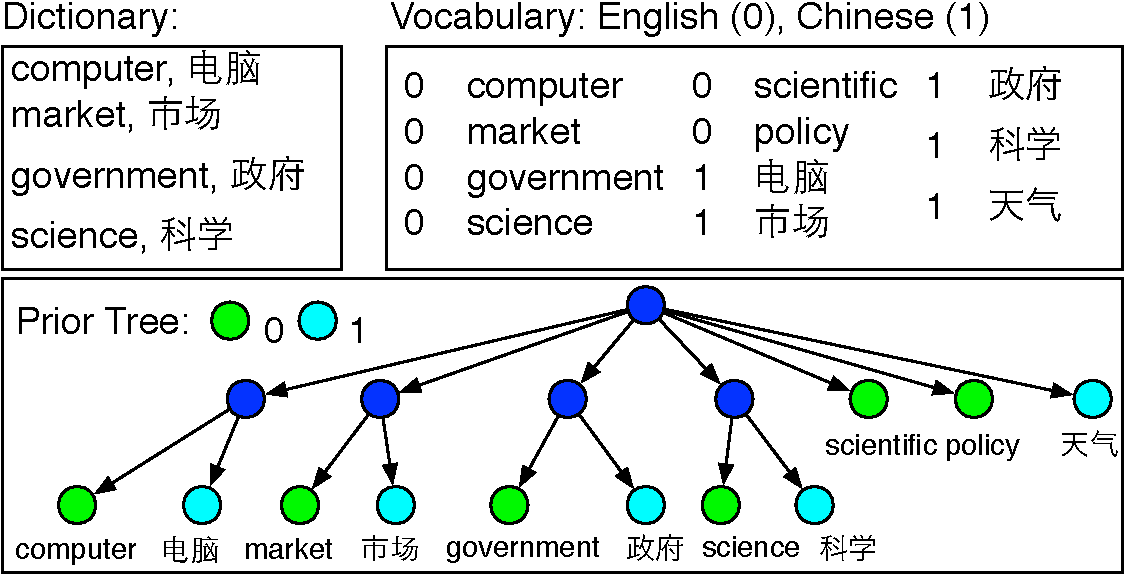
\includegraphics[width=0.9\linewidth]{figures/correlations_tree-crop.pdf}
\vspace{-3mm}
\caption[Constructing prior tree from a bilingual dictionary]{An example of constructing a prior tree from a
  bilingual dictionary: word pairs with the same meaning but in
  different languages are concepts; a common parent node is created to
  group words in a concept, and then is connected to the root;
  uncorrelated words are connected to the root directly.}
\label{fig:prior_trees}
\end{figure}

The probability of a path in a topic depends on the transition
probabilities in a topic.  Each concept $i$ in topic $k$ has a
distribution over its child nodes that is governed by a Dirichlet prior:
$\pi_{k,i} \sim \text{Dir}(\beta_{i})$.  Each path ends in a word
(i.e., a leaf node) and the probability of a path is the product of
all of the transitions between topics it traverses. Topics have
correlations over words because the Dirichlet parameters can encode
positive or negative correlations~\citep{andrzejewski-09}.

As a result, to sample a word $w_{dn}$ given a topic $z_{dn}$, a path
$y_{dn}$ from the topic tree of topic $z_{dn}$ is sampled: we start
from the root $n_0$ and first sample a child node $n_1$ of the root;
if node $n_1$ is a concept node, we continue to sample a word node
$n_2$ and generate the word associated with $n_2$; if node $n_1$ is a
word node already, we generate the word directly.

\jbgcomment{Give intuition, e.g. selecting a concept first and then
  you get the language-specific version. \yhcomment{added.}}

When this tree serves as a prior for topic models, words in the same
concept are positively correlated in topics.  For example, if
``\begin{CJK*}{UTF8}{gbsn}电脑\end{CJK*}'' has high probability in a
  topic, so will ``computer'', since they share the same parent
  node. With the tree priors, each topic is no longer a distribution
  over word types; instead, it is a distribution over paths, and each
  path is associated with a word type.  The same word could appear in
  multiple paths, and each path represents a unique sense of this
  word.



\jbgcomment{Would be nice if the prior tree were multilingual.  Would
  also be good to give back pointer to the interaction section where
  it's also discussed \yhcomment{fixed.}}

\section{Alignment from Parallel Corpora and Lexical Information}

Bilingual dictionaries and other sources of word-level information are 
valuable in training multilingual models, because they can easily specify 
simple lexical relationships that might be difficult to extract from parallel corpora.
But such manually generated data may be brittle, low-quality, or missing contextual differences in actual usage.
These two approaches are not mutually exclusive, however; they reveal
different connections across languages. \citet{hu-14} bring existing
tree-based topic models~(\tlda{}) and polylingual topic
models~(\plda{}) together and create the polylingual tree-based topic
model~(\ptlda{}) that incorporates both word-level correlations and
document-level alignment information.

To build up the prior tree structure, \citet{hu-14} consider two
resources that correlate words across languages. The first is
multilingual dictionaries, which match words with the same meaning in
different languages together. The other is the word alignments
extracted from aligned sentences in a parallel corpus. These relations
between words are used as the concepts~\citep{Bhattacharya-2006} in
the prior tree (Figure~\ref{fig:prior_trees}).

Given the prior tree structure, the generation of documents is a
combination of \tlda{} and \plda{}.  For each aligned document pair
$(d_{l_1}, d_{l_2})$, we first sample a distribution over topics
$\theta_d$ from a Dirichlet prior $\text{Dir}(\alpha)$.  For each
token in the aligned document $d_{l_i}$, we first sample a topic
$z_{dn}$ from the multinomial distribution $\theta_d$, and then sample
a path $y_{dn}$ along the tree of topic $z_{dn}$. Because every path
$y_{dn}$ leads to a word $w_{dn}$ in language $l_{dn}$, we append the
sampled word $w_{dn}$ to document $d_{l_{dn}}$ in language $l_{dn}$.

If we use a flat symmetric Dirichlet prior in place of the tree prior,
the model is equivalent to \plda{}. Similarly, if all documents are monolingual (i.e., with
distinct distributions over topics $\theta$), the model is equivalent to\tlda{}. \ptlda{} connects different languages on both the word
level (using the word correlations) and the document level (using the
document alignments), thus it learns better topics by considering more
information from both languages.


\section{Topic Models and Machine Translation}

The most frequent application of multilingual topic models is in machine translation.
Given a text input in one language (source language), statistical
machine translation tries to find a similar sequence of words in another
language (target language). Modern machine translation
systems~\citep{koehn-09} use millions of training examples to learn
the translation rules and apply these rules on the test data. 
Topic models are useful in this application when they can help to inform word meaning and word choice in specific contexts.
While the translation rules are learned in local context, these systems work
best when the training corpus has a consistent \emph{domain}, such as a
 genre (e.g., sports, business) or style (e.g.,
newswire, blog-posts). 

Translations within one domain are better than translations across
domains since they vary dramatically in their word choices and style.
A correct translation in one domain may be inappropriate in another
domain.  For example, ``\begin{CJK*}{UTF8}{gbsn}潜水\end{CJK*}'' in the
  \underline{sports} domain usually means ``underwater diving'', but
  in the \underline{social media} domain, it means a non-contributing
  ``lurker''. To avoid such translation errors caused by a domain
  change, domain knowledge is needed to train translation systems that
  are robust to such systematic variation in the training set, which
  are said to exhibit \emph{domain adaptation}.

To train such \textsc{smt} systems with domain adaptation, early
efforts focus on building separate models given the hand-labeled
domains~\citep{foster-07,matsoukas-09,chiang-11}. However, this setup
is at best expensive and at worst infeasible for large data.  Topic
models provide a promising solution where domains can be automatically
discovered. Each extracted topic is treated as a soft
domain.\footnote{Henceforth we will use the term ``topic'' and
  ``domain'' interchangeably: ``topic'' to refer to  a word distribution in
  topic models and ``domain'' to refer to \textsc{smt} corpora.} Thus
the normal monolingual topic models trained only on the source documents have
been applied to extract domain knowledge for machine
translation~\citep{Eidelman-12}.

However, the source language the and target language can complement
each other to build up more accurate topic models. For example, if we
only know the Chinese phrase ``\begin{CJK*}{UTF8}{gbsn}潜
  水\end{CJK*}'', it is hard to decide whether it is a
  \underline{sport} domain or it is a \underline{social media}
  domain. However, with the help of the aligned English translation
  ``lurker'', it is easy to identify the ``social media'' domain. Thus
  multilingual topic models~\citep{ni-09,DeSmet-09,mimno-09,boyd-graber-10} have been
  applied to extract domain knowledge for machine
  translation~\citep{hu-14}.

\section{The Components of Statistical Machine Translation}

Statistical machine translation represents translation as a
combination of probabilistic processes, a phrase-level translation model and a sentence-level language model~\citep{koehn-03,koehn-09}. 
Topic models have been applied to both aspects of this process.
Given a source sentence $\mathbf{f}$, the best
translation in target language $\mathbf{e}_\texttt{best}$ is
\begin{equation}
\mathbf{e}_\texttt{best} = \textbf{argmax}_\mathbf{e} p(\mathbf{e}|\mathbf{f}) = \textbf{argmax}_\mathbf{e} p(\mathbf{f}|\mathbf{e}) p (\mathbf{e}),
\end{equation}
which is split to a \textit{translation model}
$p(\mathbf{f}|\mathbf{e})$ and a \textit{language model} $p
(\mathbf{e})$.
Intuitively, a good translation should be both a good match for the source sentence (scoring high in the translation model) and a good sentence in its own right (scoring high in the language model).

In the \textit{decoding} phase, the source sentence $\mathbf{f}$ is segmented into multiple source
phrases $\bar{f}_n$, which are translated to a set
of target phrases $\bar{e}_n$. Thus the translation probability
$p(\mathbf{f}|\mathbf{e})$ can be further decomposed to the phrase
translation probability $p(\bar{f}_n | \bar{e}_n)$.
In the \textit{reordering} phase target phrases may then need to be repositioned to get the best
translation result. Reordering is captured by a relative distortion
probability distribution $d(a_n - b_{n-1})$, where $a_i$ denotes the
start position of the source phrase that was translated to the $n$th
target phrase, and $b_{n-1}$ denotes the end position of the source
phrase translated into the $(n-1)$th target phrase. As a result, the
translation model can be decomposed as,
\begin{equation}
p(\mathbf{f}|\mathbf{e}) = \prod_{n} p(\bar{f}_n | \bar{e}_n) d(a_n - b_{n-1})
\end{equation}

In phrase-based \textsc{smt}, the phrase probability $p(\bar{f}_n |
\bar{e}_n)$ can be further estimated by combining lexical translation
probabilities of words contained in that phrase~\citep{koehn-03},
which is normally referred as \textit{lexical weighting}. Lexical
conditional probabilities $p_w(f|e)$ are maximum likelihood estimates
from relative lexical frequencies,
\begin{equation}
\label{eq:lexical_prob}
p_w(f|e) = \textstyle \slfrac{c(f, e)}{\sum_f{c(f, e)}}
\end{equation}
where $c(f, e)$ is the count of observing lexical pair $(f, e)$ in the
training dataset. Given a word alignment $a$, the lexical weight for
this phrase pair $p_w(\bar{f} | \bar{e}; a)$ is the normalized product
of lexical probabilities of the aligned word pairs within that phrase
pair:
\begin{equation}
\label{eq:phrase_prob}
p_w(\bar{f} | \bar{e}; a) = \prod_{i} \frac{1}{\{|j | (i, j) \in a\}|} \sum_{\forall (i,j) \in a} p_w(f_i | e_j)
\end{equation}
where $i$ and $j$ are the word positions in target phrase $\bar{e}$
and source phrase $\bar{f}$ respectively.

Next we introduce how to apply topic models to improve translation
models, language models, and reordering models respectively.


\section{Topic Models for Phrase-level Translation}
\label{sec:trans-multiling}

Translation models map words and phrases from one language to another.
Both monolingual topic models and bilingual topic models are useful for improving translation models.
The most prominent application of topic models is in {\em domain adaptation}.

To train such \textsc{smt} systems with domain adaptation, early
efforts focus on building separate models based on hand-labeled
domains~\citep{foster-07,matsoukas-09,chiang-11}. For example, for all
the training examples that are labeled as \underline{sports} domain, we get 
one translation model. Continuing the earlier example, in any test document
that is labeled as \underline{sports}, ``\begin{CJK*}{UTF8}{gbsn}潜
  水\end{CJK*}'' will always be translated as ``underwater diving'', and
  the probability of translating ``\begin{CJK*}{UTF8}{gbsn}潜
    水\end{CJK*}'' as ``lurker'' is zero. In fact, such hard domain
    labels are not only expensive and time consuming to obtain, but
    also unsmoothed and sensitive to labeling errors and inconsistency: someone may lurk in a sports forum, and someone may share stories about diving on social media.

Hard domain labels are difficult to apply and can decrease the robustness of translations: domains are fundamentally uncertain, and if you get the domain wrong, you may cut off useful information.
Topic models provide a way of automatically discovering soft domain
assignments. 
If we equate the $K$ topic distributions over the vocabulary in a topic model with $K$ 
\textsc{smt} domains, each document's topic distribution can be viewed as a soft
domain assignment for that document.
If there
are two topics \underline{sports} and \underline{social media} and
a test example is most likely about \underline{sports}, it may
have a soft domain distribution as $85\%$ for \underline{sports}
domain and $15\%$ for \underline{social media} domain. These automatically
obtained soft domain labels are well smoothed, and they are not only
cheap to obtain but also much more robust to topic errors. 
We next describe applications of monolingual and multilingual
topic models to improve translation models~\citep{Eidelman-12,hu-14}.

\jbgcomment{Give an example of Chiang's hard domain assignment and
  then give an example of how topic models can do this using ``soft''
  assignment.  Then go into the mathematical
  details. \yhcomment{added.}}

%\subsection{Translation Domain Adaptation with Topic Models}


%Given the soft domain assignments, \citet{Eidelman-12} extract
%lexical weighting features conditioned on the topics, optimizing
%feature weights using the \emph{Margin Infused Relaxed
%Algorithm}~\cite[\textsc{mira}]{Crammer:2006}.  The topics come from
%source documents \emph{only} and create topic-specific lexical
%weights from the per-document topic distribution $p(k|d)$, which is
%used to smooth the expected count $\hat{c}_{k}(f,e)$ of a word
%translation pair under topic $k$,

\paragraph{Translations from monolingual topic models}

We can train a translation model by counting the frequency of pairs from word-level alignment data.
\citet{Eidelman-12} builds topic-specific translation models by reweighting the frequency of word pairs based on soft topic/domain assignments for documents.
Since a translated document is assumed to have the same topics in both languages, we only require a monolingual topic model trained on one or the other language.
The document-topic distribution $p(k|d)$ is used
to smooth the expected count $\hat{c}_{k}(f,e)$ of a word translation
pair under topic $k$,
\begin{align}
\textstyle \hat{c}_{k}(f,e) = \sum_{d}{p(k|d)c_d(f,e)},
\end{align}
where $c_d(\bullet)$ is the number of occurrences of the word pair in
document $d$.  The lexical probability conditioned on topic $k$ is the
unsmoothed probability estimate of those expected counts
\begin{align}
\label{eq:lexical_prob_k}
\textstyle p_w(f|e;k) = \hat{c}_{k}(f,e) / \sum_f{\hat{c}_{k}(f,e)},
\end{align}
from which we can compute the lexical weight of this phrase pair
$p_w(\bar{f}|\bar{e};a, k)$ given a word alignment $a$ \citep{koehn-03}:
\begin{align}
\label{eq:phrase_prob_k}
p_w(\bar{f} | \bar{e};a, k) = \prod^{n}_{i=1} \frac{1}{\{|j | (i, j) \in a\}|} \sum_{\forall (i,j) \in a} p_w(f_i | e_j; k)
\end{align}
where $i$ and $j$ are the word positions in target phrase $\bar{e}$
and source phrase $\bar{f}$ respectively. 
Equations~\ref{eq:lexical_prob_k} and \ref{eq:phrase_prob_k} are equivalent to Equations~\ref{eq:lexical_prob} and ~\ref{eq:phrase_prob}, but with the addition of soft topic/domain assignments.
\citet{Eidelman-12} combines the standard $f(\bar{f}|\bar{e})$ and
$f(\bar{e}|\bar{f})$ with two directions of
topic-adapted probabilities 
$p_w(\bar{f} | \bar{e};a, k)$ and $p_w(\bar{e} | \bar{f};a, k)$, equivalent to introducing $2K$ new word translation tables. 
Feature weights are optimized through
using the Margin Infused Relaxed
  Algorithm (MIRA)~\cite[\textsc{mira}]{Crammer-06}.

For a test document $d$, the document topic distribution $p(k | d)$ is
inferred based on the topics learned from training data. The lexical
weight feature of a phrase pair $(\bar{f}, \bar{e})$ is,
\begin{align}
\textstyle f_{k}(\bar{f}|\bar{e})=-\log\left\{{p_{w}(\bar{f}|\bar{e};k)\cdot p(k|d)}\right\},
\end{align}
a combination of the topic dependent lexical weight and the topic
distribution of the document, from which we extract the phrase.

These adapted features allow us to bias the translations according to
the topics. For example, if topic $k$ is dominant in a test document,
the feature $f_k(\bar{f} | \bar{e})$ will be large, which may bias the
decoder to a translation that has small value of the standard feature
$f(\bar{f}|\bar{e})$. In addition, combining the adapted features with
the standard features makes this model more flexible. For a test
document with less clear topics, the topic distribution will tend
toward being fairly uniform. In this case, the topic features will
contribute less to the translation results and the standard features
will dominate the translation results.

%\paragraph{Topical Lexical and Phrasal Features}

%\citet{hasler-12} also apply monolingual topic models for domain adaptation to
%\textsc{smt} in a similar framework as \citet{Eidelman-12}, except
%they introduce different features which they call sparse word pair
%features and phrase pair features. The topics on source documents are
%integrated as a source side trigger for a particular word pair or
%phrase pair as sparse features. For example, given a word $w_f$ with
%topic $k$, for an aligned word pair $(w_f, w_e)$ which is observed $c$
%times in the aligned sentence pair, the sparse word pair feature $wp$
%with topics is represented as $wp\_k\_w_f \sim w_e = c$, while the
%original word pair feature is $wp\_w_f \sim w_e = c$. The topic phrase
%pair features are also defined in a similar way: given an aligned
%phrase pair $(p_f, p_e)$ with count $c$ in the same sentence, the
%sparse phrase pair feature $pp$ with topics is represented as
%$pp\_k\_p_f \sim p_e = c$. Both the phrase pair and word pair features
%are extracted from the aligned training sentence pairs, and then
%\textsc{mira} is used to learn the feature weights.
%
%One difference in \citet{hasler-12} from \citet{Eidelman-12} is that
%they are using \emph{hidden topic Markov
%  models}~\citep[\textsc{htmm}]{gruber-07} instead of \textsc{lda} to
%learn topics. While \textsc{lda} assumes that each word is generated
%independently in a document, \textsc{htmm} models the word topic in a
%document as a Markov chain where all words in a sentence are assigned
%with the same topic. \textsc{htmm} computes $p(z_n, \Phi_n | d, w_1,
%\cdots, w_N)$ for each sentence, where $z_n$ is the topic of sentence
%$n$ in document $d$, $w_1, \cdots, w_N$ are the words in the sentence
%$n$, $\Phi_n$ is the topic transition between words. $\Phi_n$ is only
%non-zero at sentence boundaries. The advantage of using \textsc{htmm}
%is that each sentence gets the same topic assignment, thus the topic
%for each phrase pair in the aligned sentence is consistent and can be
%used for topical features directly.


\citet{hasler-12} also apply monolingual topic models for domain adaptation to
\textsc{smt} in a similar framework as \citet{Eidelman-12}, except
they apply \emph{hidden topic Markov models}~\citep[\textsc{htmm}]{gruber-07} 
instead of \textsc{lda} to learn topics and extract different features. 
While \textsc{lda} assumes that each word is generated
independently in a document, \textsc{htmm} models the word topic in a
document as a Markov chain where all words in a sentence are assigned
with the same topic. As a result, the topic
for each phrase pair in the aligned sentence is consistent and can be
used for topical features directly.

%\paragraph{Topical Phrase Probability via Topic Mapping}

\citet{su-12} use \textsc{htmm} to incorporate topic information
into the phrase probability directly, rather than through the word
translation probability.
Given the bilingual translation
training data without any specific domain information (referred as
out-of-domain bilingual data), they incorporate topic information
from the source language into translation probability estimation, and
decompose the phrase probability $p(\bar{e}|\bar{f})$ as,
\begin{align}
p(\bar{e}|\bar{f}) = \sum_{k_{out}} p(\bar{e}, k_{out} | \bar{f}) = \sum_{k_{out}} p(\bar{e} | \bar{f}, k_{out})  \cdot p(k_{out} | \bar{f})
\end{align}
where $p(\bar{e} | \bar{f}, k_{out})$ is the translation probability given 
the source side topic $k_{out}$, and $p(k_{out} | \bar{f})$ denotes the 
phrase probability in topic $k_{out}$.

Besides, \citet{su-12} assume that a monolingual corpus in the
same domain as the test sentence (referred to as in-domain monolingual
data) is available. Thus they also apply \textsc{htmm} to estimate the
in-domain topic $k_{in}$ and $p(k_{in} | \bar{f})$.  However, the
in-domain topics $k_{in}$ and the out-of-domain topics $k_{out}$ may
not be in the same space, so \citet{su-12} introduce the topic mapping
probability $p(k_{out} | k_{in})$ to map the in-domain topic to the
out-of-domain topic:
\begin{align}
p(k_{out} | \bar{f}) = \sum_{k_{in}} p(k_{out} | k_{in}) \cdot  p(k_{in} | \bar{f})
\end{align}
As a result, the final phrase probability can be refined as,
\begin{align}
p(\bar{e}|\bar{f}) = \sum_{k_{out}} \sum_{k_{in}} p(\bar{e} | \bar{f}, k_{out}) \cdot p(k_{out} | k_{in}) \cdot p(k_{in} | \bar{f})
\end{align}
The topic and topic mapping relationship
between the training data and test data can be built offline, so the
whole process adds no additional burden to the translation system.

Monolingual topic models can add contextual information about word choice to 
translation models, but do not by themselves take advantage of multilingual information.
We next turn to topic models that explicitly learn multilingual connections between words.

\paragraph{Multilingual Information for Domain Adaptation}

Using bilingual data adds modeling complexity, but can also improve topic model quality.
One can think of topic models as tools for disambiguating the meaning of words based on their context. 
Aligning across multiple languages is a common way of resolving such ambiguities.
 For example, ``\begin{CJK*}{UTF8}{gbsn}木马\end{CJK*}'' in a Chinese
  document can be either ``hobbyhorse'' in a \underline{children}'s
  topic, or ``Trojan virus'' in a \underline{technology} topic.  
  A monolingual topic model might not be able to tell the difference in a short Chinese document, but these terms
  are unambiguous in English, more accurately indicating the relevant topic.

%Multilingual topic models have been shown to improve results in \textsc{smt} \citep{hu-14}.
%There are various ways to build up the multilingual topic
%models. Different languages can be connected on the
%word-level~\citep{boyd-graber-07,andrzejewski-09,hu-14:itm} or the
%document levels~\citep{mimno-09}, or a combination of both \citep{hu-14}. 

While many of the approaches described in this chapter try to model the source and target
languages simultaneously to extract topics, some of the benefit of multilingual models can be achieved by aligning monolingual models. \citet{xiao-12} apply
topic models on the source documents and target documents separately
to learn the document-topic distributions $p(k_f | d_f)$ and $p(k_e |
d_e)$, and then estimate the phrase-topic probabilities $p(\bar{e}, k_f
| \bar{f})$ and $p(\bar{e}, k_e | \bar{f})$ from each model. They further
compute the topic similarity scores between the phrase topic
distribution and document topic distribution as features for decoding
to improve \textsc{smt} results.

To translate a new document $d_f$, they first estimate the document-topic distribution $p(k_f |
d_f)$.
Then for a given phrase $\bar{f}$ in the source document they search for the target phrase $\bar{e}$ that maximizes the similarity between the source document's topic distribution $p(k_f|d_f)$ and the phrase-topic distribution $p(\bar{e}, k_f|\bar{f})$ according to squared Hellinger distance $H^2(p,q) = \sum_k \left(\sqrt{p_k} - \sqrt{q_k} \right)^2$.
Second, they calculate a projection between the two monolingual topic models $p(k_f
| k_e)$  by normalizing the co-occurrence count in the aligned training
sentences, and use this relationship to calculate the conditional distribution of target phrases and target topics $p(\bar{e}, k_e|\bar{f})$.

This topic projection idea is similar to the topic mapping by
\citet{su-12}, but it is applied between the source language and the
target language. Compared to the lexical features in
\citet{Eidelman-12} and \citet{hu-14}, \citet{xiao-12} introduce a new
framework to apply topic information directly to measure the relationship between phrases and present two topic similarity features for decoding. These two approaches can
be combined to further improve \textsc{smt}.

\section{Topic Models for Sentence-level Language Modeling}


A critical component of machine translation systems is the language
models, which provide local constraints and preferences to make
translations more coherent. A language model describes the probability
of a word $w$ occurring given the previous context words, which is
also mentioned as the history $h$. We have introduced the application
of language models in information retrieval in
Chapter~\ref{sec:ir-lm}. In fact, it also helps to choose the correct
or more proper word during the statistical machine translation. For
example, the English words ``house'' and ``home'' are in many cases synonymous, but the translation ``I am going home'' is better than
``I am going house''.

Domain adaptation for language models~\citep{Bellegarda-04,wood-09}
uses extra knowledge to adjust this probability $p(w|h)$ to reflect
the content change, which is an important avenue for improving machine
translation. As \citet{Bellegarda-04} points out, ``an adaptive
language model seeks to maintain an adequate representation of the
current task domain under changing conditions involving potential
variations in vocabulary, syntax, content, and style''.

Topics from topic models can be one of the resources to provide such
knowledge for language model adaptation. For example, the Chinese
phrase ``\begin{CJK*}{UTF8}{gbsn}很多粉丝\end{CJK*}'' is translated to
  ``a lot of vermicelli'' in a \underline{food} domain, but means ``a
  lot of fans'' in an \underline{entertainment} domain. Such ambiguity
  can be reduced by using topic/domain knowledge. If the \underline{entertainment} topic is extracted based on
  the previous context, this Chinese phrase will be translated to ``a
  lot of fans'' without any ambiguity. Next, we introduce the details
  about applying topic models for language model adaptation.

\paragraph{Language Model Adaptation from Monolingual topic models}

Early work~\citep{Clarkson-1997,Seymore-1997,Kneser-1997,Iyer-1999} focuses on
partitioning the training data to multiple topic-specific subsets and
building up language models for each subset. Then the topic-specific
language models $p_k(w|h)$ are linearly combined with a general
language model $p_g(w|h)$ built from all training data as
Equation~\ref{eq:linear_lm}. The weights $\lambda_k$ can be tuned
based on the topics of the test documents.
\begin{align}
\label{eq:linear_lm}
p_\textrm{adapted}(w|h) = \sum_k \lambda_k p_k(w|h) + \lambda_g p_g(w|h)
\end{align}

\citet{Seymore-1998} further identify the most appropriate topic for
each word in the vocabulary and choose either a topic-specific language model
or the general language model. The intuition is that the general
language model provides the most reliable estimation for general
words, and the topic language model estimates the probability more
accurately for more specific words. As a result, they split the vocabulary
words into three groups: the general subset, on-topic subset and
off-topic subsets. They use the general language model for the general subset and the off-topic subset and the topic-specific language model for  the
on-topic subset.

All of these methods use a traditional n-gram model, which conditions on a finite, bounded history.
These models also assume each document or history belongs
to exactly one topic cluster.
To fix these problems, models with topic mixtures, such as
\emph{Latent Semantic Analysis}~\citep[\textsc{lsa}]{deerwester-90}
and its probabilistic interpretation probabilistic latent semantic
indexing (pLSI)~\citep[\textsc{plsi}]{hofmann-99},
learn large-span language
models~\citep{Bellegarda-1997,Coccaro-1998,Gildea-1999}. \citet{Gildea-1999}
decomposes the language model based on topics,
\begin{align}
\label{eq:plsi_lm}
p(w|h) = \sum_k p(w|k) p(k|h)
\end{align}
where the topics are learned from the training corpus by optimizing the log probability,
\begin{align}
l(\theta; N) = \sum_w \sum_d n(w,d) \log \sum_k p(w|k) p(k|d)
\end{align}
where $d$ is the training documents, and $n(w,d)$ is the word frequency of $w$ in document $d$. $p(w|k)$ and $p(k|d)$ are learned through the EM algorithm. For test documents, they fix $p(w|k)$ to estimate $p(k|h)$ and then compute $p(w|h)$ using Equation~\ref{eq:plsi_lm}. 

This way of applying topic models to language models is 
similar to document language modeling for information retrieval
as in Chapter~\ref{sec:ir-lm}. However, unlike
information retrieval, two different languages are involved in the
process of \textsc{smt}, and they can complement each other to learn
more accurate topics. Next, we discuss multilingual topic models
for language model adaptation.

\paragraph{Language Model Adaptation from Multilingual Topic Models}

As we explained in Section~\ref{sec:trans-multiling}, the information
from different languages can complement each other to extract better
topics. Latent semantic models such as LSA have been used in multilingual information retrieval for many years \cite{carbonell1997translingual}.
In order to introduce multilingual information to probabilistic topic models
for language model adaptation, various approaches such as
\cite{Tam-2007}, \cite{Ruiz-2011}, \cite{Yu-2013} etc., have been
explored. 

\cite{Tam-2007} introduces the bilingual latent semantic
analysis~(\textsc{blsa}) to learn the topics for both source language
and target language, and apply the learned topics into language model
adaptation for \textsc{smt}. Similar to polylingual topic models~\citep{mimno-09}, 
\textsc{blsa} transfers the inferred
topics from the source language to the parallel target language.

More specifically, \cite{Tam-2007} assume the aligned source document
and the target document share the same document-topic distribution.
They first learn an \textsc{lsa} model on the source
language and then use the document-topic vector from the
source document as the document-topic vector for the aligned
target document, and then infer the topic-word vector on the
target side. The topics for the target language are not learned
iteratively, thus the topics in a parallel corpus can be learned very
efficiently.

In order to apply the topics for language adaptation, the word
marginal distribution $p_{lsa}(w)$ for document $d$ is computed,
\begin{align}
p_{lsa}(w) = \sum_{k=1}^K p(w|k) p(k|d)
\end{align}
Then this word marginal distribution is integrated into the target background language model by minimizing the KL divergence between the adapted language model and the background language model~\citep{Kneser-1997b}:
\begin{align}
\label{eq:mdi}
p_a(w|h) \propto \Big( \frac{p_{lsa}(w)}{p_{bg}(w)} \Big) ^{\beta} \cdot p_{bg}(w|h)
\end{align}

\cite{Ruiz-2011} apply a similar idea for language model
adaptation. Instead of using \textsc{blsa}, \cite{Ruiz-2011} simply
merge the aligned source and target document as one document, and
train pLSI. Both ideas are
based on the assumption that the aligned source document and target
document share the same document-topic distribution. The final adapted
language model combines the topic-based language model with the
general background language model, thus it is more robust in improving
the results of \textsc{smt}.

\jbgcomment{again, good to have ex}

\citet{Yu-2013} presents a hidden topic Markov model~(\textsc{htmm}) to improve
the language model in \textsc{smt}. They build up a topic model on the
source side and target side respectively, and learn a topic-specific
language model based on the target side by estimating the
maximum-likelihood. To smooth the sharply distributed probabilities,
back-off probabilities are also considered as follows:
\begin{align}
p(w_i | w^{i-1}_{i-n+1}, k_e) = &\lambda_{w^{i-1}_{i-n+1}} p_{MLE}(w_i|w^{i-1}_{i-n+1}, k_e) \\
&+ (1- \lambda_{w^{i-1}_{i-n+1}})p_{MLE}(w_i|w^{i-1}_{i-n+2}, k_e)
\end{align}
where $\lambda$ is the normalization parameter, calculated by,
\begin{align}
\lambda_{w^{i-1}_{i-n+1}, k_e} = \frac{N_{1+}(w^{i-1}_{i-n-1},
  k_e)}{N_{1+}(w^{i-1}_{i-n-1}, k_e) + \sum_{w_i}c(w^i_{i-n+1}, k_e)}
\end{align}
where $N_{1+}(w^{i-1}_{i-n-1}, k_e)$ is the number of words following
$w^{i-1}_{i-n-1}$ in topic $k_e$, and $c(w^i_{i-n+1}, k_e)$ is the
count of n-gram $w^i_{i-n+1}$ in $k_e$.

During the decoding, since no target sentence is available, they extract the topics on the 
source side and project the source topic to the target side. 
The target probability is estimated as following:
\begin{align}
p(e) = \sum_{k_e} p(e|k_e) p(k_e) = \sum_{k_e} p(e|k_e) \cdot \sum_{k_f} p(k_e|k_f) p (k_f)
\end{align}
where $p(k_e|k_f)$ is the topic projection probability, estimated by
the co-occurrence of the source-side and the target-side topic assignment.


\section{Reordering with Topic Models}

In addition to translation models and languages models, a third
important component of a phrase-based \textsc{smt} systemt is 
reordering models, which learn how the order of words in the source
sentences influences the order of words in the target sentences and
how to make the translations in the right order.
The usefulness of topic models in reordering is less clear than their usefulness 
for domain adaptation of translation models
and language models, but it is nevertheless significant.
The primary advantage is that word order in different domains of the same
language may be different: \citet{Chen-2013} find that training corpora in different domains vary
significantly in their reordering characteristics for particular
phrase pairs.
As the example shown in
Table~\ref{tab:reorder-topic}~\citep{wang-14}, in an \underline{economy}
topic, the Chinese word \begin{CJK*}{UTF8}{gbsn}比\end{CJK*} is on the
  left of \begin{CJK*}{UTF8}{gbsn}五\end{CJK*}; but in a
    \underline{sports} topic, \begin{CJK*}{UTF8}{gbsn}比\end{CJK*} is
      on the right of \begin{CJK*}{UTF8}{gbsn}五\end{CJK*}. As a
        result, it is necessary to introduce domain knowledge
        to model such order variance, and topic models provide a good data-driven way to do so.

\begin{table}[!tp]
\begin{center}
\setlength\tabcolsep{3pt}
\begin{tabular}{c || c c} \hline
Topic & Type & Example \\ \hline \hline
\multirow{2}{*}{Economy} & Source & $\cdots$ \textbf{\begin{CJK*}{UTF8}{gbsn}比五\end{CJK*}} \begin{CJK*}{UTF8}{gbsn}月份下降\end{CJK*}$3.8\%$ $\cdots$\\
                     & Target & $\cdots$ down $3.8\%$ from May $\cdots$\\ \hline
\multirow{2}{*}{Sports} & Source & $\cdots$ \textbf{\begin{CJK*}{UTF8}{gbsn}五比\end{CJK*}}\begin{CJK*}{UTF8}{gbsn}一\end{CJK*}$3.8\%$ $\cdots$\\
                     & Target & $\cdots$ five to one $\cdots$\\ \hline
\end{tabular}
\caption{Topics influence the word orders: the Chinese words in bold
  are in different orders in different topics. (Example from
  \citet{wang-14})}
\label{tab:reorder-topic}
\end{center}
\end{table}

\citet{Xiong-2006} treat the
reordering problem as a classification with two labels: straight and
inverted between two consecutive blocks, and build up a maximum
entropy classification model as the reordering model.
\citet{Chen-2013} manually divide the training data into
multiple domains, instead of using automatic techniques such as topic
models.
\citet{wang-14} integrate two more types of
topic-based features into the reordering model, in additional to the
boundary word features used in \citet{Xiong-2006}. First, they choose
the topic with maximum probability in a document to be the
\textit{document topic feature} for that document. Besides, they also
use the topics of the content words that locate at the left and
rightmost positions on the source phrases as the \textit{word topic
  features} to capture topic-sensitive reordering patterns.

During the decoding process, \citet{Xiong-2006} infer the topic
distributions of the test documents first and then apply this proposed
topic-based reordering model as one sub-model to the log-linear maximum entropy model
to obtain the best translation:
\begin{align}
e_\texttt{best} = \texttt{argmax}_e \Big \{ \sum_{m=1}^M \lambda_m h_m(e,f) \Big \}
\end{align}
where $h_m(e,f)$ are the sub-models or features of the whole
log-linear model, $\lambda_m$ are their weights accordingly, which are
tuned on the development set.

This framework is very flexible and can encode any topic-based features.
Any multilingual topic models we have discussed so far can be
applied to extract better topics.



%The goal of a lexicalized reordering model is to learn the orientation
%probabilities for a given phrase pair with respect to the previous
%phrase pair and the following phrase pair~\citep{Chen-2013}. The
%orientation $o$ typically includes three types: monotone (M), swap (S)
%and discontinuous (D). The M orientation means the current phrase pair
%is immediately to the right of the previously translated phrase in the
%source sentence, S orientation occurs when the current phrase is
%immediately to the left of the previous phrase, and all other cases
%all belong to D orientation.
%The model is ``lexicalized'' because the estimated orientations depend on the words in both the
%previously translated phrase pair and the current phrase pair.
%
%Formally, the reordering model is defined to estimate the
%corresponding probabilities $p(o|f,e)$ using recursive MAP smoothing:
%\begin{align}
%p(o|f,e) &= \frac{c(o,f,e) + \alpha_f p(o|f) + \alpha_e p(o|e)}{c(f,e) + \alpha_f + \alpha_e} \\
%p(o|f) &= \frac{c(o,f) + \alpha_g p(o)}{c(f) + \alpha_g} \\
%p(o|e) &= \frac{c(o,e) + \alpha_g p(e)}{c(e) + \alpha_g} \\
%p(o) &= \frac{c(o) + \alpha_u/3}{c(\cdot) + \alpha_u}
%\end{align}
%where $c(o,f,e)$ is the orientation counts obtained from the word-aligned corpus;  the parameters $\alpha_f$, $\alpha_e$, $\alpha_g$ and $\alpha_u$ are learned by minimizing the perplexity of the resulting model on the held-out data.
%
%\citet{Chen-2013} find that training corpora in different domains vary
%significantly in their reordering characteristics for particular
%phrase pairs, thus they introduce a linear model for adapting reordering
%models. Given $N$ sub-corpora (or $N$ domain corpus), they
%first train a reordering model on each domain-specific corpus, and then define
%the global reordering model as a linear combination of the reordering
%models on each domain corpus:
%\begin{align}
%p(o|f,e) = \sum_{i=1}^{N} \alpha_i p_i(o|f,e)
%\end{align}
%where $p_i(o|f,e)$ is the reordering model on sub-corpus $i$, and the weight $\alpha_i$ are learned by maximizing the probability of phrase-pair orientations in the in-domain development set:
%\begin{align}
%\hat{\alpha} = \texttt{argmax}_{\alpha} \sum_{o,f,e} \tilde{p}(o,f,e) \log \sum_{i=1}^N \alpha_i p_i(o|f,e)
%\end{align}
%where $\tilde{p}(o,f,e)$, proportional to $c(o,f,e)$, is the empirical distribution of counts in the development set. \citet{Chen-2013} propose to smooth the in-domain sample and weight instances by document frequency to further improve the mixture adaptation. They demonstrate this adaptation significantly improve the statistical machine translation system.
%
%However, \citet{Chen-2013} manually divide the training data into
%multiple domains, instead of using automatic techniques such as topic
%models. \citet{wang-14} apply topic models to maximum entropy
% phrase reordering models \citep{Xiong-2006}.
%
%Under the ITG constraints~\citep{wu-1997}, three Bracketing
%Transduction Grammar (BTG) rules are used to constrain the translation
%and reordering:
%\begin{align}
%A &\rightarrow [A^1, A^2]\\
%A &\rightarrow <A^1, A^2>\\
%A &\rightarrow f/e
%\end{align}
%where $A$ is a block with a pair of source and target strings; $A^1$
%and $A^2$ are two consecutive blocks; the two rules are reordering
%rules which merge two blocks into a larger block in a straight or
%inverted order. Rule 3 translates a source phrase $f$ to a target
%phrase $e$ and generate a block $A$. These three rules applied until the whole source sentence is covered, generating a 
%hierarchical segmentation tree of the source sentence in the process.
%
%Based on this hierarchical setting, \citet{Xiong-2006} treat the
%reordering problem as a classification with two labels: straight and
%inverted between two consecutive blocks, and build up a maximum
%entropy classification model as the reordering model:
%\begin{align}
%p(o|c(A^1, A^2)) = \frac{\exp(\sum_i \theta_i f_i(o, c(A^1, A^2)))}{\sum_{o'} \exp(\sum_i \theta_i f_i(o', c(A^1, A^2)))}
%\end{align}
%where $\theta_i$ are the feature weights, $c(A^1, A^2)$ indicates the attributes of $A^1$ and $A^2$, and $f_i(o, c(A^1, A^2))$ are binary features defined as,
%\begin{align}
%f_i(o, c(A^1,A^2)) = \begin{cases}
%1, &\text{if $(o,c(A^1, A^2))$ satisfies certain condition} \\
%0, &\text{else}
%\end{cases}
%\end{align}
%
%This framework only uses the features extracted from the blocks
%instead of the whole block (in contrast to lexicalized reordering),
%thus it is flexible to reorder any blocks~\citep{Xiong-2006}.




\section{Beyond Domain Adaptation}

In addition to translation models, language models and reordering models,
there are also other modules of \textsc{smt}, such as word alignment,
where topic models have also been applied. \citet{zhao-06} present a
Bilingual topical admixture (BiTAM) to improve  word
alignment in \textsc{smt}. BiTAM assumes each document pair is an
admixture of topics, and the topics for each sentence pair within that
document pair are sampled from the same document-topic
distribution. Each topic also has a topic-specific translation
table. Therefore, the sentence-level word alignment and translations
are coupled by the hidden topics.  BiTAM captures the latent
topical structure and generalizes word alignments and translations via
topics shared across sentence pairs, thus the quality of the
alignments is improved.

Besides, coherence, which ties sentences of text into a meaningfully
connected structure~\citep{xiong-13}, is another important piece to
\textsc{smt}. \citet{xiong-13} introduce a topic-based coherence model
to improve the document translation quality. They learn the sentence
topic for source documents, based on which they predict the target
topic chain; they then incorporate the predicted target coherence
chain into the document translation decoding process.

In general, multilingual topic models obtain topics with high quality,
since different languages can complement each other to reduce topic
ambiguity. Many different approaches, have been explored to apply such
multilingual topic models to improve different pieces of statistical
machine translation. With such topic knowledge, the variations of
different languages can be better captured to make the translations
more natural and coherent.



\chapter{Conclusion}
\label{ch:conc}

While we have attempted to cover a variety of the applications of
topic models to help individuals navigate large text datasets, no
finite survey could enumerate all of the applications of topic models
in text, which have been applied to part of speech
tagging~\citep{toutanova-08}, word sense induction~\citep{brody-09},
and entity disambiguation~\citep{kataria-11}.  It goes without saying
that we have also omitted many other applications outside text, such
as biology~\citep{pritchard-00}, understanding source
code~\citep{maskeri-08}, music analysis~\citep{hu-09}, and many more.

\section{Coping with Information Overload}
\label{sec:fast-inference}

A challenge in topic modeling is how to make inference efficient
enough to both scale to large datasets and to provide low-latency
interactive experiences to help provide support to a user in the loop.
Three broad directions support this efficient learning of large topic
models.  There are three broad strategies for processing documents
more quickly.

% TODO Add in something about document-centric perspective (anchors, etc)

The first is through decreasing the average number of times a computer
needs to look at a document to learn a topic model; i.e., to improve
\emph{throughput}.  Online algorithms~\cite{hoffman-10} only look at a
document once, update the topics, and then move on to the next
document.  This is often much faster than batch approaches which
require many passes over the same set of documents.  Another option is
to \emph{distribute} computation across many machines~\citep{zhai-12}.

A complementary approach is to reduce the time a computer spends on
any particular document: improving \emph{efficiency}.  This is
possible by improving how long it takes to sample document
assignments~\citep{yao-09,li2014reducing} or compute variational
parameters~\citep{mimno-12}.

The final approach to improve the efficiency of probabilistic
algorithms for topic models is to rethink the inference process
entirely.  Novel approaches view topic model inference as a
factorization of a co-occurence matrix~\citep{arora-13} or as a spectral
decomposition~\citep{anandkumar-12}.  These approaches often are much faster than
traditional approaches as they use word types---rather than
documents---as the central unit of computation.

\section{Deeper Representations}

Part of the benefit of topic models is that the topic distribution of
a document ($\theta$) serves as a low-dimensional representation of
what the document means.  This numerical vector is useful for finding
similar documents (Chapter~\ref{ch:ir}), displaying documents to a user
(Chapter~\ref{ch:viz}), or connecting documents across languages
(Chapter~\ref{ch:mt}).

Increasingly, vector-based representations have been useful ``all the
way down''.  Vector-based representations of words and phrases can
improve next word prediction~\citep{bengio-03}, sentiment
analysis~\citep{socher-12}, and translation~\citep{devlin-14}.  And
this is not just for text---representation learning has taken hold of
speech, vision, and machine learning generally.

The impact of representation learning on topic modeling remains
unclear as we go to press in 2017.  We see several ways that
representation learning and topic modeling could benefit each other in
the future.

\paragraph{Evaluation}

Evaluation methods from topic models have made their way into
representation learning, which suggests that some of the lessons
learned in making topic models interpretable (Section~\ref{ch:viz}) could
also be applied in representation learning.  This could help mollify
some critics of representation learning who argue that the results are
often uninterpretable or deceptive~\citep{szegedy-13}.

\paragraph{Synthesis}

Topic modeling is also blending with more expressive latent
representation models~\citep{ranganath-15}.  Topic models could help
representation learning solve some of its difficulty summarizing
larger segments of text.  Paragraphs and sentences are difficult to
model as a single vector, and techniques more sophisticated than
simple averaging don't seem worth the hassle~\citep{iyyer-15}.

\paragraph{Parallel Evolution}

Another possible path is less intertwined: topic models and
deep-learning representation learning solve different problems and 
are not directly competitive.  Topic models offer advantages of speed and
interpretability, while representation learning can do better for
prediction-based tasks. 
Topic models have never been ideal, for example, in inducing features for text classification: it is almost always better to simply use word-count features.
If interpretability and recognizability is not a fundamental goal of your analysis, you are probably better off using something else.
However, in cases where interpretability and recognition are the main and final goals of analysis, deep learning methods currently offer little because their very advantage ---greater representational complexity---is also their weakness.
Both approaches should be tools that many text
miners have in their toolkit, with specific circumstances for using
either.

\section{Automatic Text Analysis for the People}

However, in our view, the primary research challenge of topic models
is not to make these models and their inference more complicated but
rather to make them more accessible.  As we have described, topic models
can help scholars and ordinary people navigate large text collections.

However, using topic models still requires extensive data and computer
skills.  Our job as information scientists is not complete until these
tools (or suitable alternatives) are available to everyone who needs
them.

This goal requires making the tools more usable.
The corpus preprocessing and vocabulary curation required of topic models is not straightforward: should we remove
non-English documents, what should we consider a document, how should
we handle metadata?  Nor are the modeling choices needed to make sense
of the data trivial: how many topics should we use, which of the many
possible models should we use, and what inference technique gives us the
best tradeoff between speed and accuracy?  Existing topic models do a
poor job of communicating what options are available to a user and
what consequences these choices have.

However, even if the process of creating a topic model becomes
intuitive, the output must also be interpretable.  Distributions
over words are the language that these models use to create
representations of document collections, but it is not how users think
about topics: they would much rather have phrases~\citep{mei-07},
sentences~\citep{smith-16}, or pictures~\citep{lau-14}.  However,
providing these representations is non-trivial and requires a deeper
understanding of a corpus than today's topic models can manage.

Finally, topic models need a more systematic investigation of how
they can assist users' workflow for typical information seeking,
organization, and management tasks.  While the applications covered in
this survey show examples of how people can use topic models from
applications from history to political science, how topic models can
augment or replace existing workflows lacks the same attention given
to---for example---search engines.

\section{Coda}

We hope that you have enjoyed our survey of topic models'
applications.  For further information, we would encourage the reader to
investigate the topic modeling
bibliography,\footnote{\url{https://mimno.infosci.cornell.edu/topics.html}}
join the topic modeling mailing
list,\footnote{\url{https://lists.cs.princeton.edu/mailman/listinfo/topic-models}},
or the book's associated webpage.


\backmatter  % references

\bibliographystyle{plainnat}
\bibliography{bib/journal-full,bib/jbg,bib/alison}

\end{document}
